\begin{comment}
\begin{figure}[h]
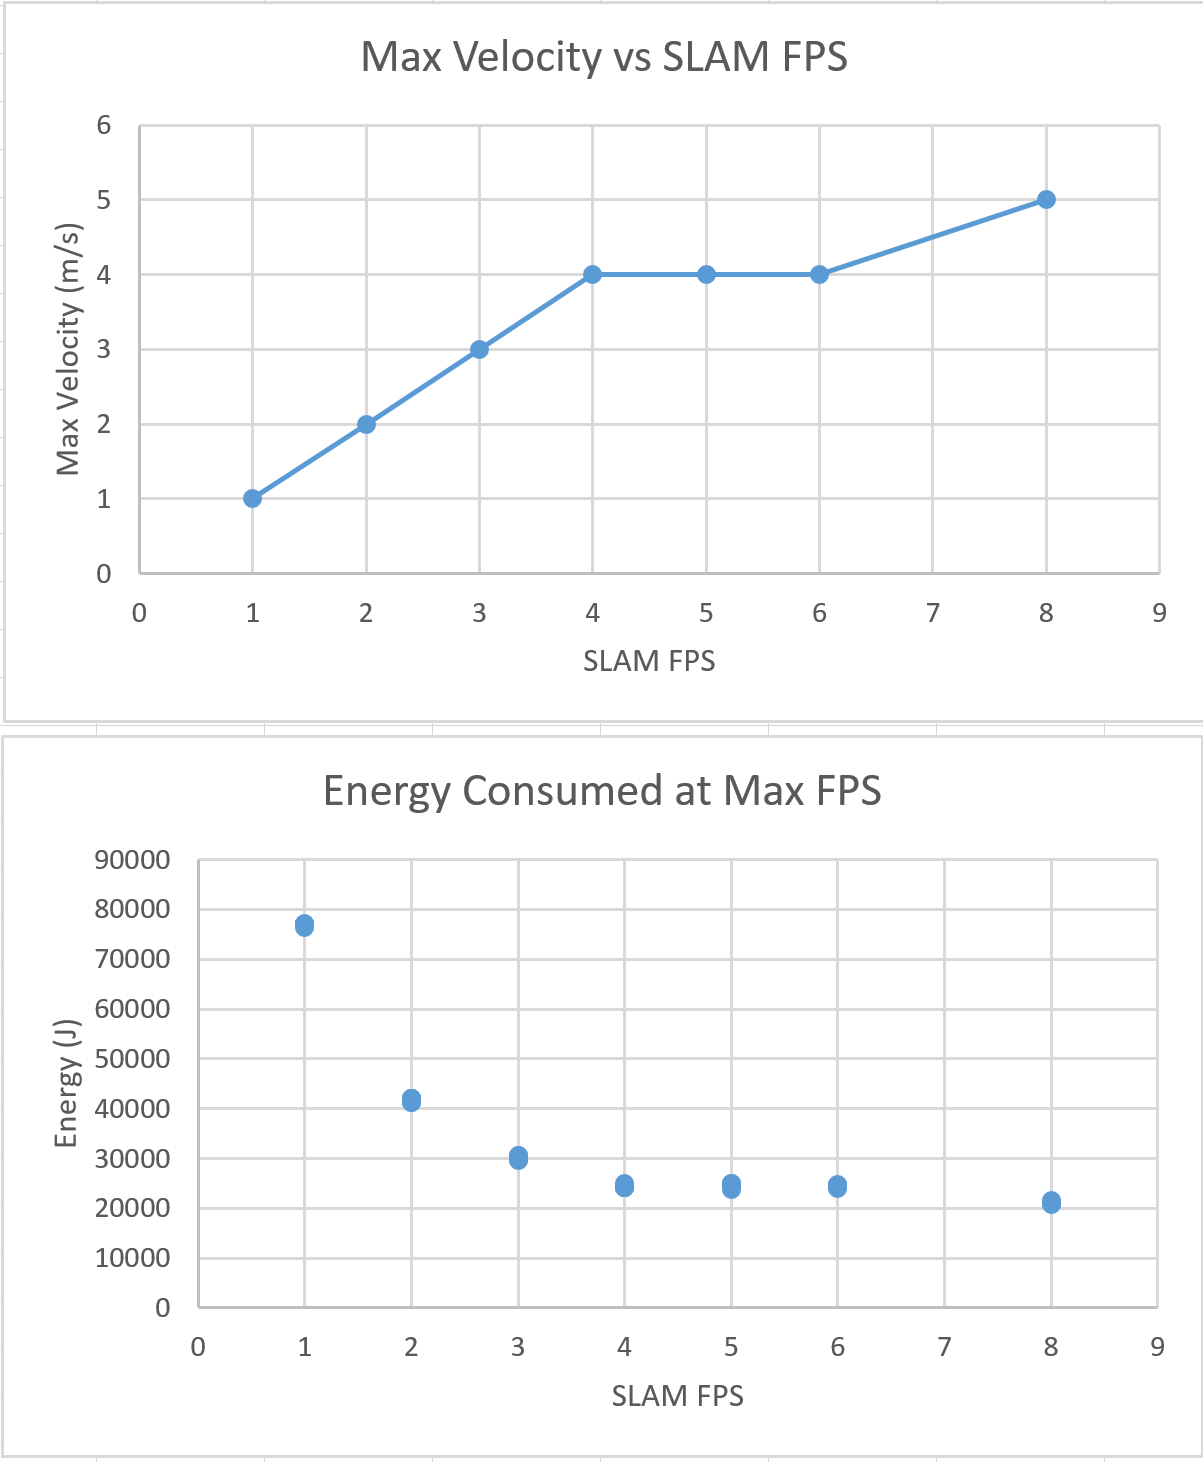
\includegraphics[width=\columnwidth]{figs/slam-speed-energy.png}
\caption{relationship between drone's speed compute power}
\label{sec:powerbreakdown}
\end{figure}
\end{comment}
\begin{comment}
\begin{figure}[h]
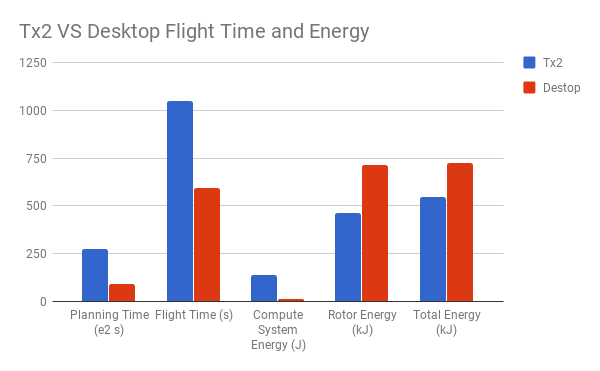
\includegraphics[width=\columnwidth]{figs/desktop_vs_tx2_mapping.png}
\caption{relationship between motion planning performance and compute power}
\label{microbenchmark_1}
\end{figure}
\end{comment}
\section{The Role of Compute in MAVs}
\label{sec:char}

In this section, we discuss how compute affects MAV systems. At the high level, compute plays a crucial role both in the overall mission time and total energy consumption of such systems. First, we discuss each effect by providing relevant  theoretical background and supplement the discussion with a microbenchmark. Then, we analyze MAVBench as a set of representative applications in which such effects can manifest.   %Figure~\ref{fig:benchmarks_data_flow} and our benchmark suits and  discuss the high level insights into aerial agents bottlenecks and their corresponding implications. 


%thout the loss of generality we use our benchmark suit to conduct studies. The results and the flow presented in section blah to explain the corresponding  the by a discussion of  total system, i.e. locomotion and compute energy consumption, and its distribution. Then, we provide case studies showing that more compute can result in an improvement in the overall system's energy consumption. Finally we delve into our application benchmark suit to discuss how such a role can effect them.

%\subsection{Compute and Accuracy Relationship}
%explain slam and present the microbenchmark

\subsection{Compute and Flight Time Relationship}

Compute can play an important role in reducing the drone's mission time by increasing the mission's average velocity. Concretely, we identify that the reduction in hover time and the increase in maximum allowed velocity are the two major ways with which more compute can contribute to a higher average velocity. Here, we shed light on these different ways.

\paragraph{Hover Time Reduction:} Hover time and the average velocity have an inverse relationship, namely, the more drone spends time on hovering, the lower its average velocity. Similar to an idling CPU, a hovering drone is unfavorable since it is not working toward its mission, but yet wasting its limited energy. A hovering drone typically is waiting for its mission planning stage to make a decision (e.g. deciding on a path to follow). \emph{More compute power can help reduce hovering (e.g by reducing the decision making time),} hence decreasing the negative effect hovering has on the average velocity. 
\begin{figure}[t!]
\centering
    \begin{subfigure}{.49\columnwidth}
    \centering
    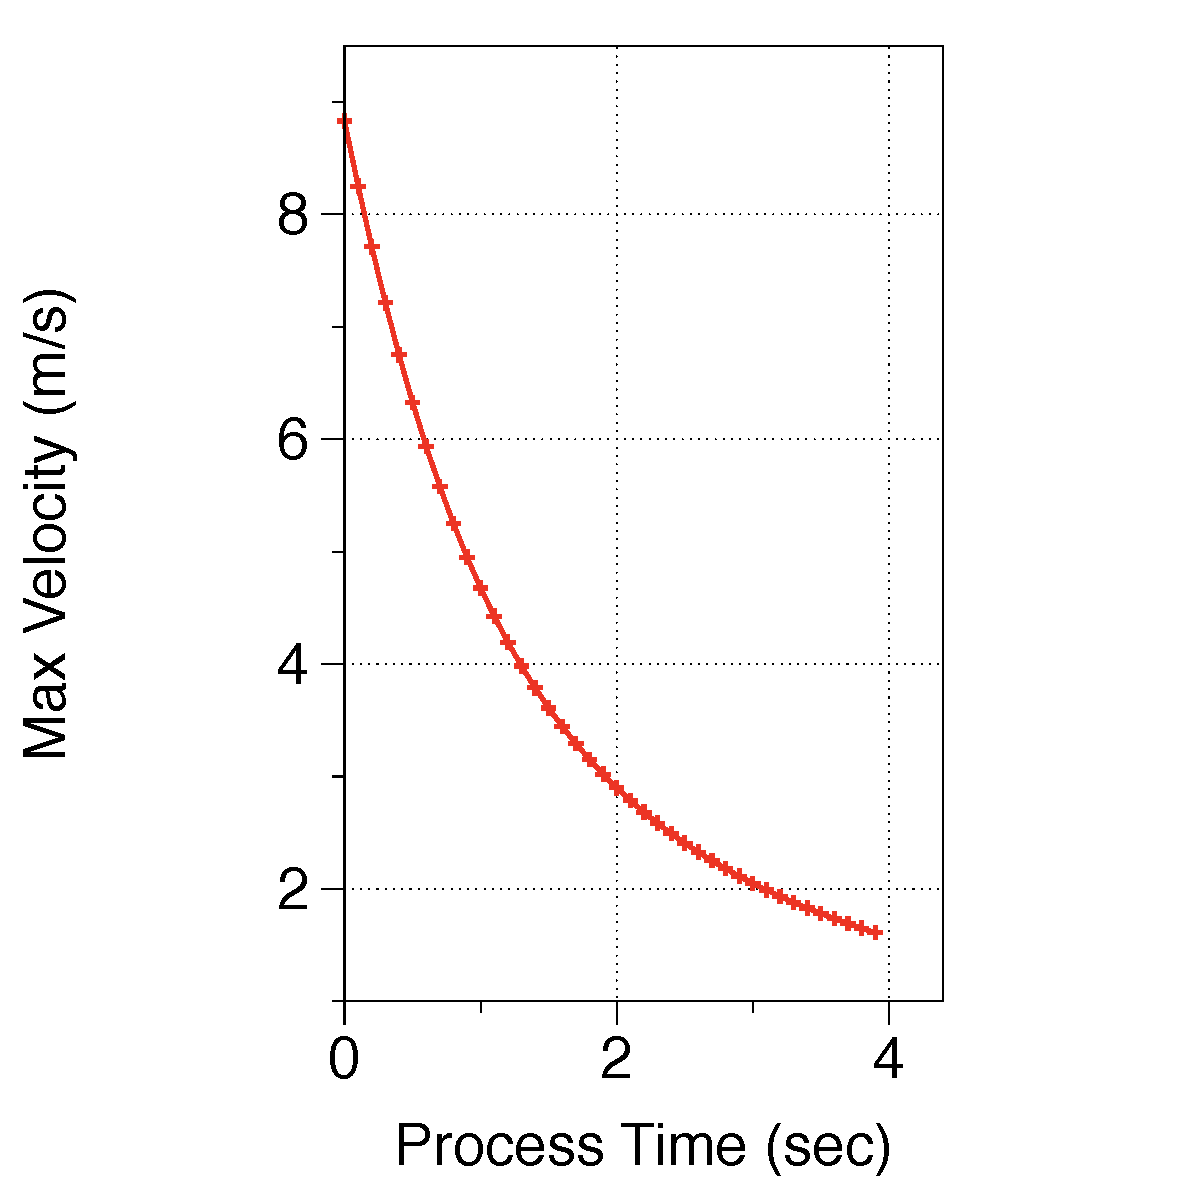
\includegraphics[trim=0 0 0 0, clip, width=1.0\columnwidth]{figs/fig_13}
    \caption{Theoretical max velocity.}
    \label{fig:process-time-velocity}
    \end{subfigure}
    \begin{subfigure}{.49\columnwidth}
    \centering
   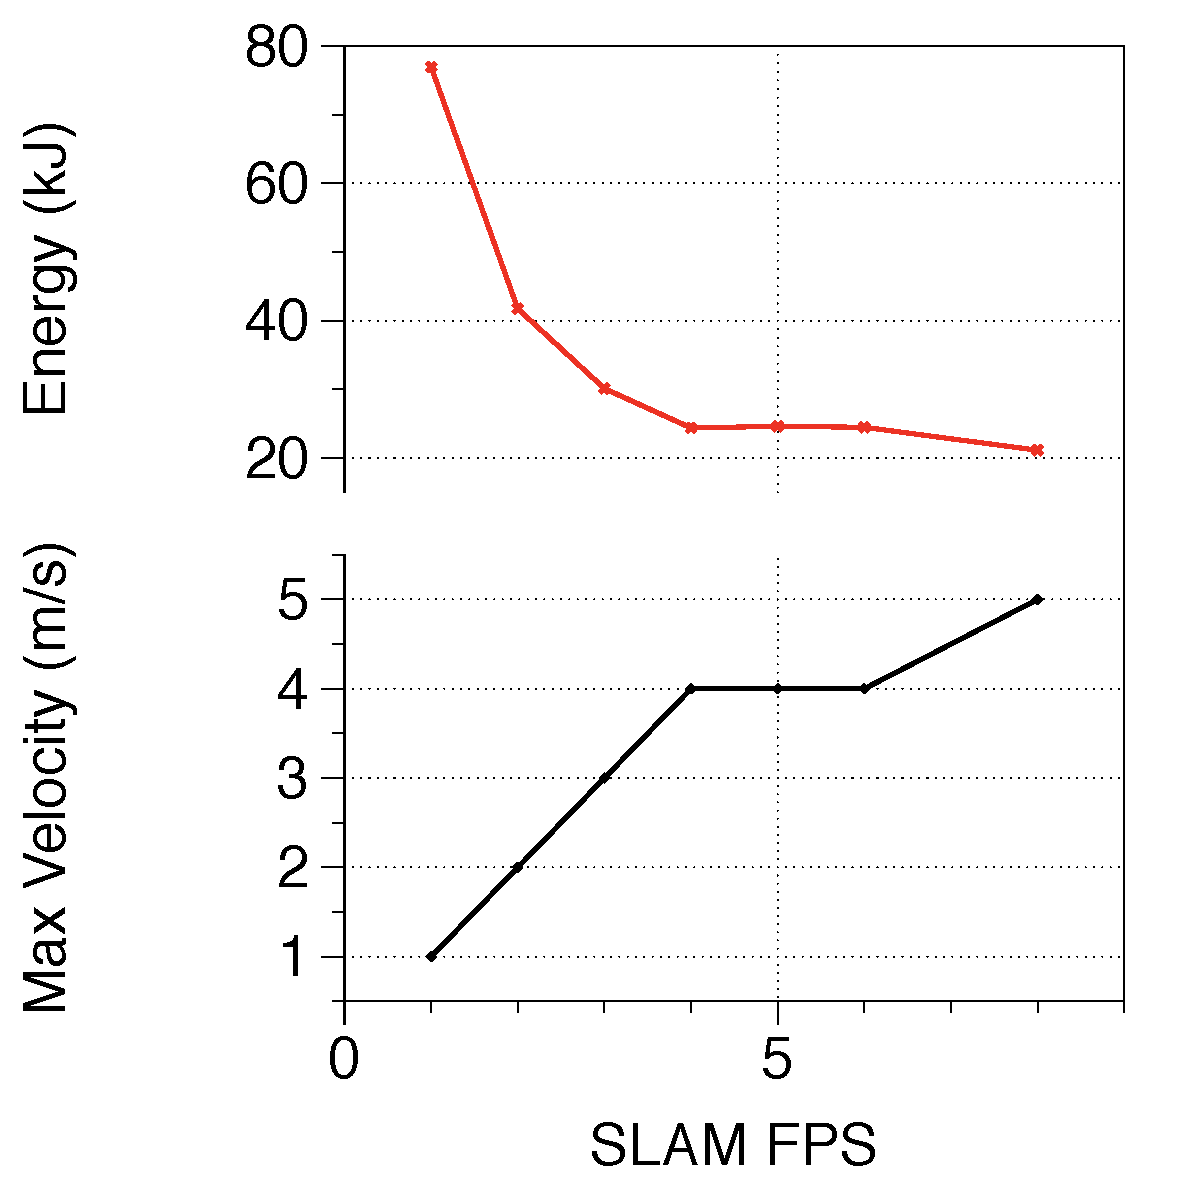
\includegraphics[trim=0 0 0 0, clip, width=1.0\columnwidth]{figs/slam_fps_velocity_energy}
    \caption{Measured max velocity.}
    \label{fig:slam-velocity-energy}
    \end{subfigure}
\vspace{-5pt}
%\setlength{\belowcaptionskip}{-4ex}
\caption{\emph{(a)} Theoretical relationship between processing time and maximum velocity. \emph{(b}) Relationship between SLAM throughput (FPS) and maximum velocity and energy of UAVs.}
%\label{SOLO_power_breakdown}
\end{figure}

\paragraph{Max Velocity Increase, Collision Avoidance Effect:} The maximum velocity of the drone is not only mechanically bounded, but also compute bounded. For a given flight velocity, a collision-free flight is only possible if the drone can process its surrounding fast enough to react to it. Therefore, \emph{a higher velocity requires a faster processing capability}. The collision avoidance task can be rather compute intensive exercising various stages of the pipeline starting from the pixel processing in the perception stage and ending with the command issue in control. In order to guarantee collision avoidance, a  drone's maximum velocity is determined based on the aforementioned pixel to response time. Equation~\ref{eq:runtime-compute-bound} specifies the components involved in setting this velocity where $\delta_{t}$, d, $a_{max}$ and v denote process time, required stopping distance, maximum acceleration limit of the drone and maximum velocity~\cite{high-speed-nav}. As \Fig{fig:process-time-velocity} shows, our simulated drone, in theory, is bounded by the max velocity anywhere between 8.83 to 1.57 m/s given a pixel to response time of the range 0 to 4~seconds. 

\begin{comment}
\begin{figure}[t]
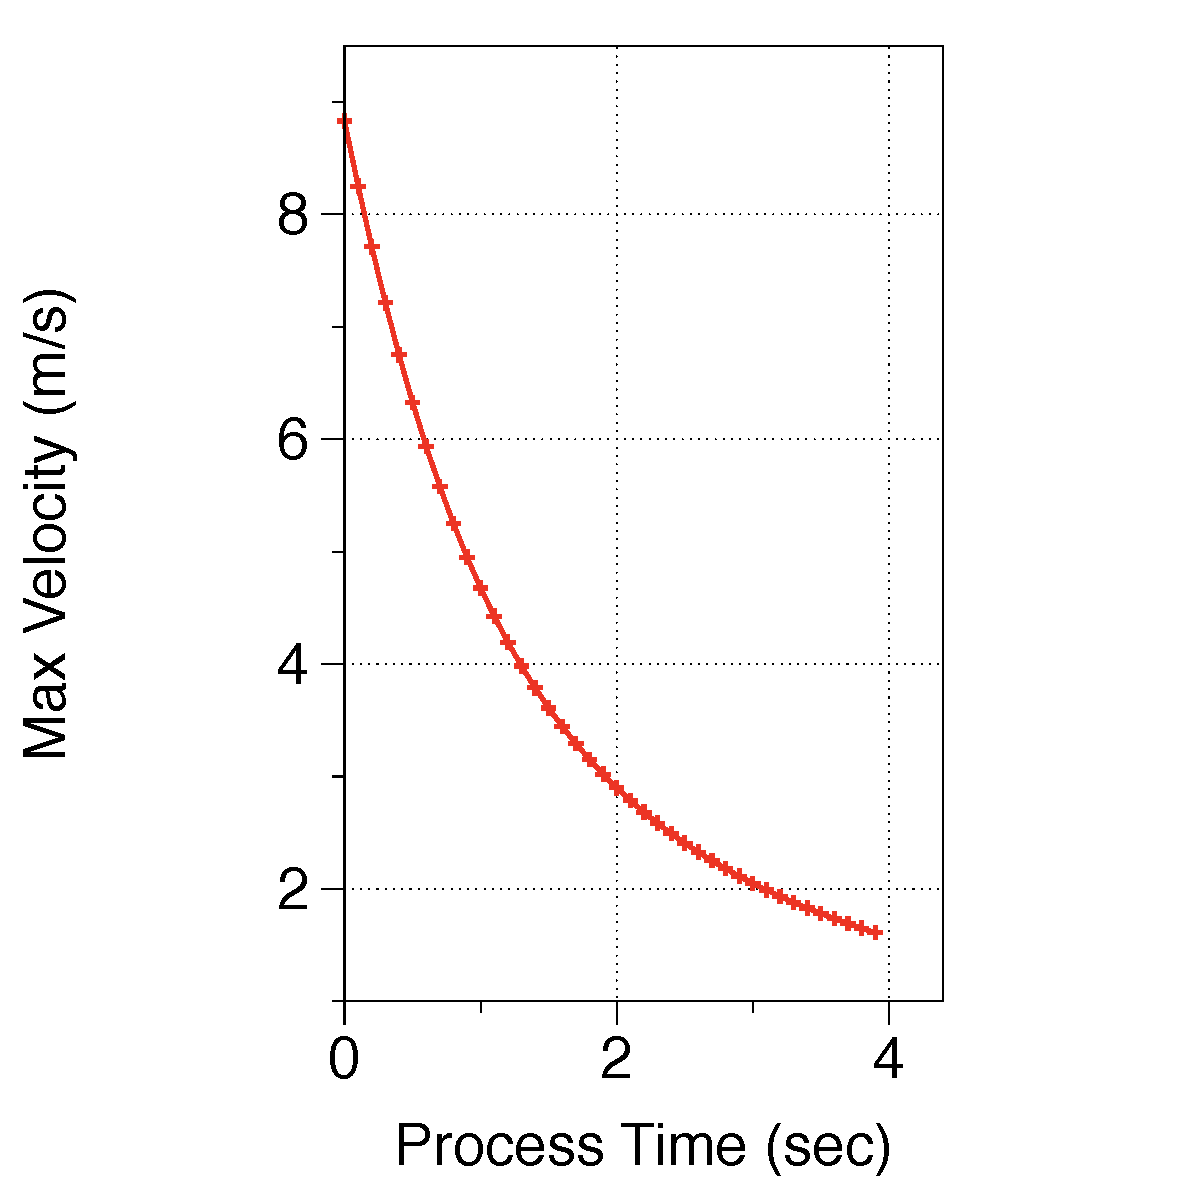
\includegraphics[width=\columnwidth]{figs/fig_13}
\caption{Theoretical relationship between process time and max velocity}
\label{sec:vel_proc_relationship_figure}
\end{figure}
\end{comment}

\begin{equation}
\label{eq:runtime-compute-bound}
v_{max} = a_{max}(~\sqrt[]{\delta{t}^2 + 2\frac{d}{a_{max}}} - \delta{t})
\end{equation}
\setlength{\belowcaptionskip}{-1ex}

\paragraph{Max Velocity Increase, Localization Failure Effect:} The faster the speed of the drone, the higher the likelihood of its localization failure because the environment changes rapidly around a fast drone. Kernels such as SLAM which help localize the drone by tracking a set of points/features through successive camera frames struggle to keep up with the rate of these changes. It is important to note that localization failures can have catastrophic effects such as permanent loss or spending of extra time (for example by backtracking) for re-localization. 

Minimizing or avoiding localization related failure scenarios is highly favorable, if not necessary. To examine the relationship between the compute, maximum velocity and localization failure, we devised a micro-benchmark in which the drone was tasked to follow a predetermined circular path of the radius 25~meters. For the localization kernel, we used ORB-SLAM2 and to emulate different compute powers, we inserted a sleep in the kernel. We swept different velocities and sleep times and bounded the failure rate to 20\%. As \Fig{fig:slam-velocity-energy} shows, higher FPS values, i.e. more compute, allows for a higher maximum velocity for a bounded failure rate. 

%\begin{figure}[h]
%\includegraphics[]{figs/blank.pdf}
%\caption{Measurement set up to collect power data for 3DR Solo.}
%\label{sec:powerbreakdown}
%\end{figure}
\begin{figure}[!t]
\centering
    \begin{subfigure}{.49\columnwidth}
    \centering
    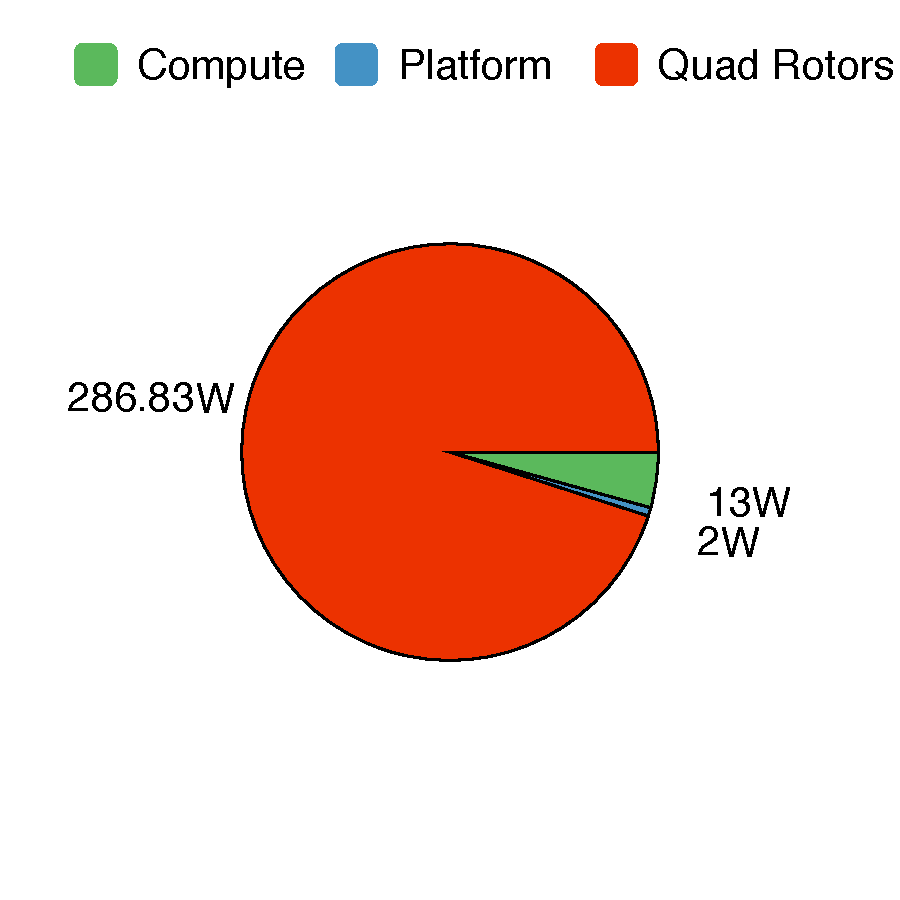
\includegraphics[trim=0 0 0 0, clip, width=1.0\columnwidth]{figs/power_break_down_tx2}
    \caption{Measured power breakdown.}
    \label{fig:SOLO-power-breakdown}
    \end{subfigure}
    \begin{subfigure}{.49\columnwidth}
    \centering
    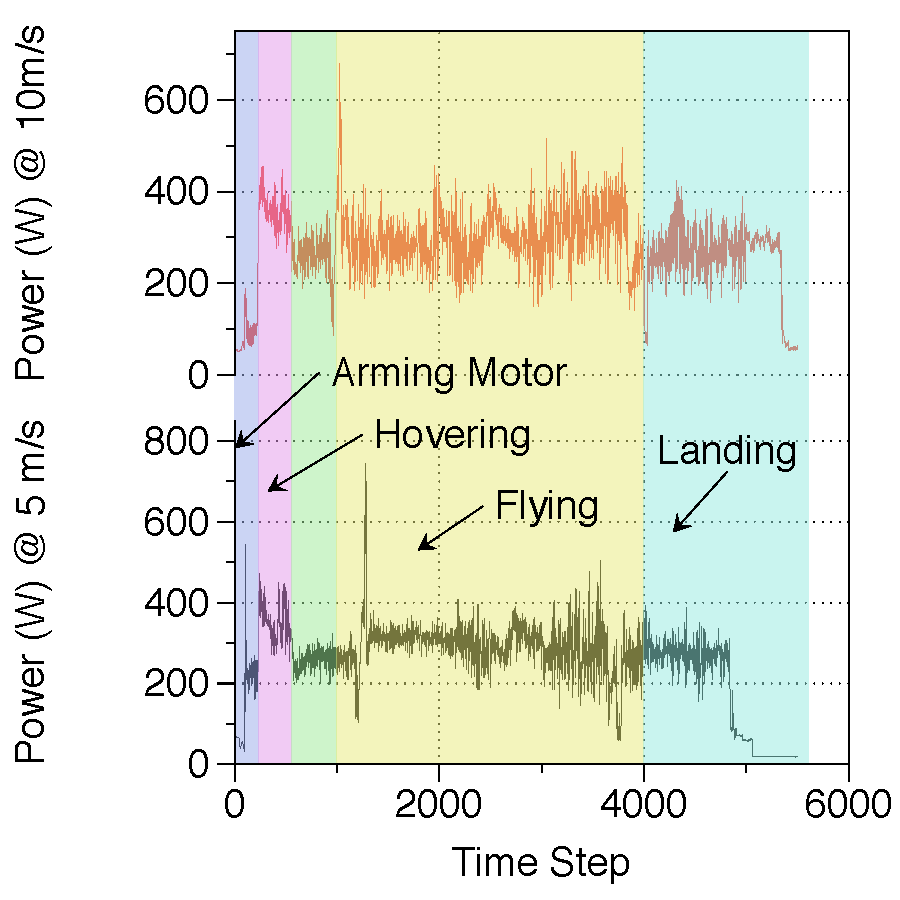
\includegraphics[trim=0 0 0 0, clip, width=1.0\columnwidth]{figs/drone-power-time-series}
    \caption{Measured mission power.}
    \label{fig:drone-power-time-series}
    \end{subfigure}
\caption{\emph{(a)} Measured power consumption of a flying 3DR Solo. \emph{(b)} Total measured power consumption while the drone is "Flying" at two different steady-state velocities. The power consumption is severely dominated by the quad rotors by 20X.}
\label{SOLO_power_breakdown}
\end{figure}
\subsection{Compute and Energy Relationship}
The compute subsystem can also have a significant role in reducing total MAV energy consumption. To understand this, first we present the power distribution associated with \solo~\cite{solo3DR}, a popular off-the-shelf MAV. To measure power, we attach a wattmeter known as Eagle~Tree Systems eLogger~V4~\cite{eLoggerV4} to the \solo's battery during flight. The wattmeter allows us to collect data over time at 50~Hz while the drone flies. We command the drone to fly for fifty seconds and pull the data off of the wattmeter after the drone lands.

% The wattmeter gave us the total power consumed by the drone, without a deeper breakdown. To estimate the portion of the instantaneous power that would typically be consumed by a MAV's processor, we subtracted the idle power consumption of the \solo's default on-board computer and added to it the power consumed by the TX2 during typical workloads.

As \Fig{SOLO_power_breakdown} shows, the majority of the power consumption is dedicated to rotors (locomotion) and the compute only occupies a small portion of the entire pie and its role seemingly trivial. Although small in quantity, compute can have a grand effect on the system's power. This is because by reducing the mission time (as explained in the previous section), more compute power can, in fact, reduce the bigger portion of the pie, namely rotors energy consumption (due to a shorter flight). Note that although more compute can lead to more energy consumption of the compute subsystem, the reduction in rotor's energy can easily outweigh such an increase.  
% \setlength{\belowcaptionskip}{-2ex}


We profiled the mission time and the energy associated with the aforementioned microbenchmark. As the bottom plot in \Fig{fig:slam-velocity-energy} shows, higher compute capability results in increased SLAM FPS and hence a reduction in mission time by allowing for faster velocity. The reduced mission results in reduced total system energy, as the top plot in \Fig{fig:slam-velocity-energy} shows. By increasing processing speed by 5X, we were able to reduce the drone's energy consumption by close to 4X.

\subsection{MAVBench Workloads Compute vs. Flight Time vs. Energy}
\label{sec:operating-spoints}
We use our benchmark suite as a representative set of applications to examine the effect of compute on MAV systems. To analyze this effect, we conducted sensitivity analysis to core and frequency scaling of the TX2 board. TX2 has two sets of cores, namely a \textit{HMP Dual Denver cores} and a \textit{Quad ARM A57}. We turned off the Denver cores so that the indeterminism caused by process to core mapping variations across runs would not affect our results.
Average velocity, mission, and energy values of various operating points are profiled and presented as heat maps (\Fig{fig:benchmarks:OPA:scanning}---\Fig{fig:benchmarks:OPA:ap}) for a DJI Matrice 100 drone. \emph{In general, compute can improve mission time and lower energy consumption by as much as 5X.}

\paragraph{Scanning:}
We observe trivial differences for velocity, endurance and energy across all three operating points (\Fig{fig:benchmarks:OPA:scanning:velocity}, \Fig{fig:benchmarks:OPA:scanning:time}, and \Fig{fig:benchmarks:OPA:scanning:energy}). This is despite seeing a 3X boost in the motion planning kernel, i.e. lawn mower planning, which is its bottleneck (\Fig{fig:kernel-breakdown}). The trivial effect of compute on this application is because planning is done once at the beginning of the mission and its overhead is amortized over the rest of the mission time. For example the overhead of planning for a 5 minute flight is less than .001\%.  
%\vspace{2pt}

%We present our understanding and takeaways regarding the computational bottlenecks and the effect of compute on them.


%Each application and its associated nodes are time profiled (table~\ref{kernel_makeup}).  We use this table along with the data flow presented in figure    \label{fig:benchmarks} to dissect and understand various compute bottlenecks. 

%At the high level, each application contains a node called mission planner responsible for high level decision making and arbitrating flight command issuance. When needed, this nodes place a service call to the motion planning kernel, setting out drones next set of moves. Some of our applications have the collision avoidance capability. This node exercises all stages of the pipeline starting from the perception stage, i.e. point cloud generation, OctoMap, collision check, to planning, mission planner/motion planner and ending with control, i.e. path tracking/command issue. 

 
%and their kernel makeup is provided. This will help us to understand the bottle-necks and opportunities for improvements.

%It would be wise to note that this application is intentionally design minimally without an involved perception and planning because ~\red{ask vijay. He knows very well how to justify this}.

\paragraph{Package Delivery}:  As compute scales with the number of cores and/or frequency values, we observe a reduction of up to 84\% and 82\% for the mission time and energy consumption, respectively (\Fig{fig:benchmarks:OPA:pd:time}, and \Fig{fig:benchmarks:OPA:pd:energy}). The sequential bottlenecks i.e. motion planning and OctoMap generation kernel are sped up by frequency scaling to enable the observed improvements. There does not seem to be a clear trend with core scaling, concretely between 3 and 4 cores. We conducted investigation and determine that such anomalies are caused by the non-real-time aspects of ROS, AirSim and the TCP/IP protocol used for the communication between the companion computer and the host. We achieve up to 2.9X improvement in OctoMap generation and that leads to maximum velocity improvement. It is important to note that although we also gain up to 9.2X improvements for the motion planning kernel, the low number of re-plannings and its short computation time relative to the entire mission time render its impact trivial. Overall the aforementioned improvements translate to up to 4.8X improvement in the average velocity. Therefore, mission time and the MAV's total energy consumption are reduced.

%OctoMap generation is a major computationally intensive kernel in this application. This kernels performance OctoMap is of utmost importance since it is on the collision avoidance path. As shown in the data flow, this path starts with depth images and flows through point cloud generation, OctoMap generation, collision check and finally ends in the control.  OctoMap is responsible for 99\% of the pixel to response time determined by this path. Figure blah shows how OctoMap kernel scales with different number of cores and frequencies. 

%Motion planner is another computationally intensive kernel for this application. Although at first glance, its optimization can improve the mission time, the low number of re-plannings and its short computation time relative to the entire mission time render its impact trivial. For example, if we re-plan 20 times during the coarse of 5 minutes of the mission time, planning time would only consume .01\% of the entire flight.  
 
\begin{comment}
\begin{figure}[h]
\includegraphics[width=\columnwidth]{figs/velocity_process_time_relationship}
\caption{Theoretical relationship between process time and max velocity}
\label{sec:vel_proc_relationship}
\end{figure}
\end{comment}

%lowering the process time, results in a higher velocity and in turn, lowering the mission time and energy. 
%Explain collision avoidance path and policty and then discuss how octomap and planning comprise most of the it and the rest is ros runtime overhead. 
%Our pixel to response time is equal to 1.2 seconds most of which is dedicated to octomap and planning as is showing in the table.   

%As opposed to the surveying benchmark, package delivery's trajectory is determined at the mission time.  perception of the obstacles surrounding the drone at any moment and also on the way to the destination is required. To do so, a map of once visible and visited environment is created and maintained within an octomap structure \ref{blah}. Arriving at such a map requires converting image depth information to point clouds (point cloud generation node) and integrating them to the map (octomap server). It is important to note the dynamic obstacles are intentional not captured within the octomap. Motion planner, attempts to find the shortest path to the destination with the knowledge of such map and only remap on demand. 
  
%As the drone follow its trajectory, new trajectory can be demanded due to environmental triggers. These environmental triggers can be static obstacles unaccounted for at the time of planning (since they were not in the sensor's visibility range). Dynamic obstacles not present at the time of planning can also trigger replannings. 

%These triggers are identified using the panic and the future collision node. The future collision node identifies whether an obstacle (mainly static ones) is on the trajectory planned and alarm the mission planner node to request a re-plan. Since future collision operates on octomap, dynamic obstacles can not be spotted to be reacted to. This is an intentional decision since dynamic obstacles can move out of the path.
%Panic node, alarms the drone of any obstacles that enters a virtual halo surrounding the drone by processing the point cloud. By equipping the drone with a forward and backward camera, we can avoid most obstacles\footnote{since each camera only has a FOV of 120 degree, there are blind spots for our drone. To fix this, more sensors are required. We address this issue in the limitation section}  This node is our solution to dynamic obstacles. In addition to dynamic obstacles, this node can save the drone from crashing in any obstacle if the control node (follow trajectory) allows for a drift from it's supposed trajectory. 

%Due to small number of replannings, the hover time associated with the planning stage has a minor affect on the mission time. In addition, small time associated with real time threads such as panic and future collision does not demand more attention. Hence, compute's role on this application is minor.

{
\begin{figure}[t!]
    	\centering
    	\begin{subfigure}[t!]{.3\columnwidth}
    	\centering
    		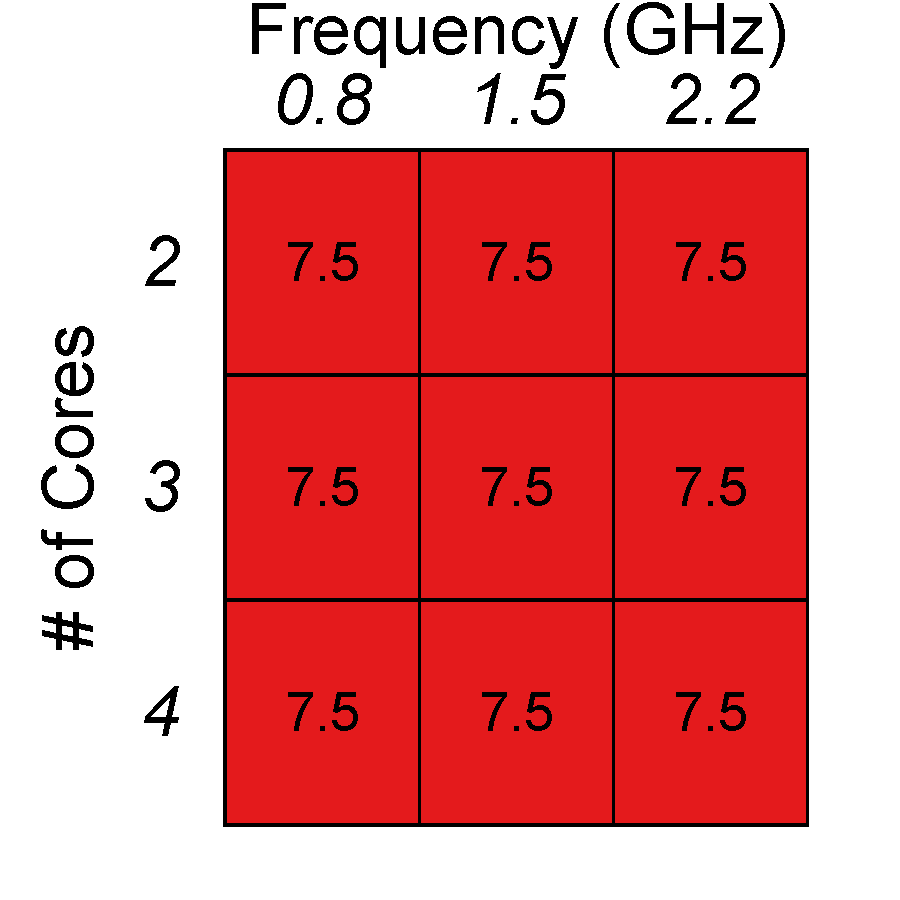
\includegraphics[width=\columnwidth]{figs/scanning_velocity_operating_point}
    		\caption{Velocity (m/s)}
            \label{fig:benchmarks:OPA:scanning:velocity}
    	\end{subfigure}
        \begin{subfigure}[t!]{.3\columnwidth}
    	\centering 
    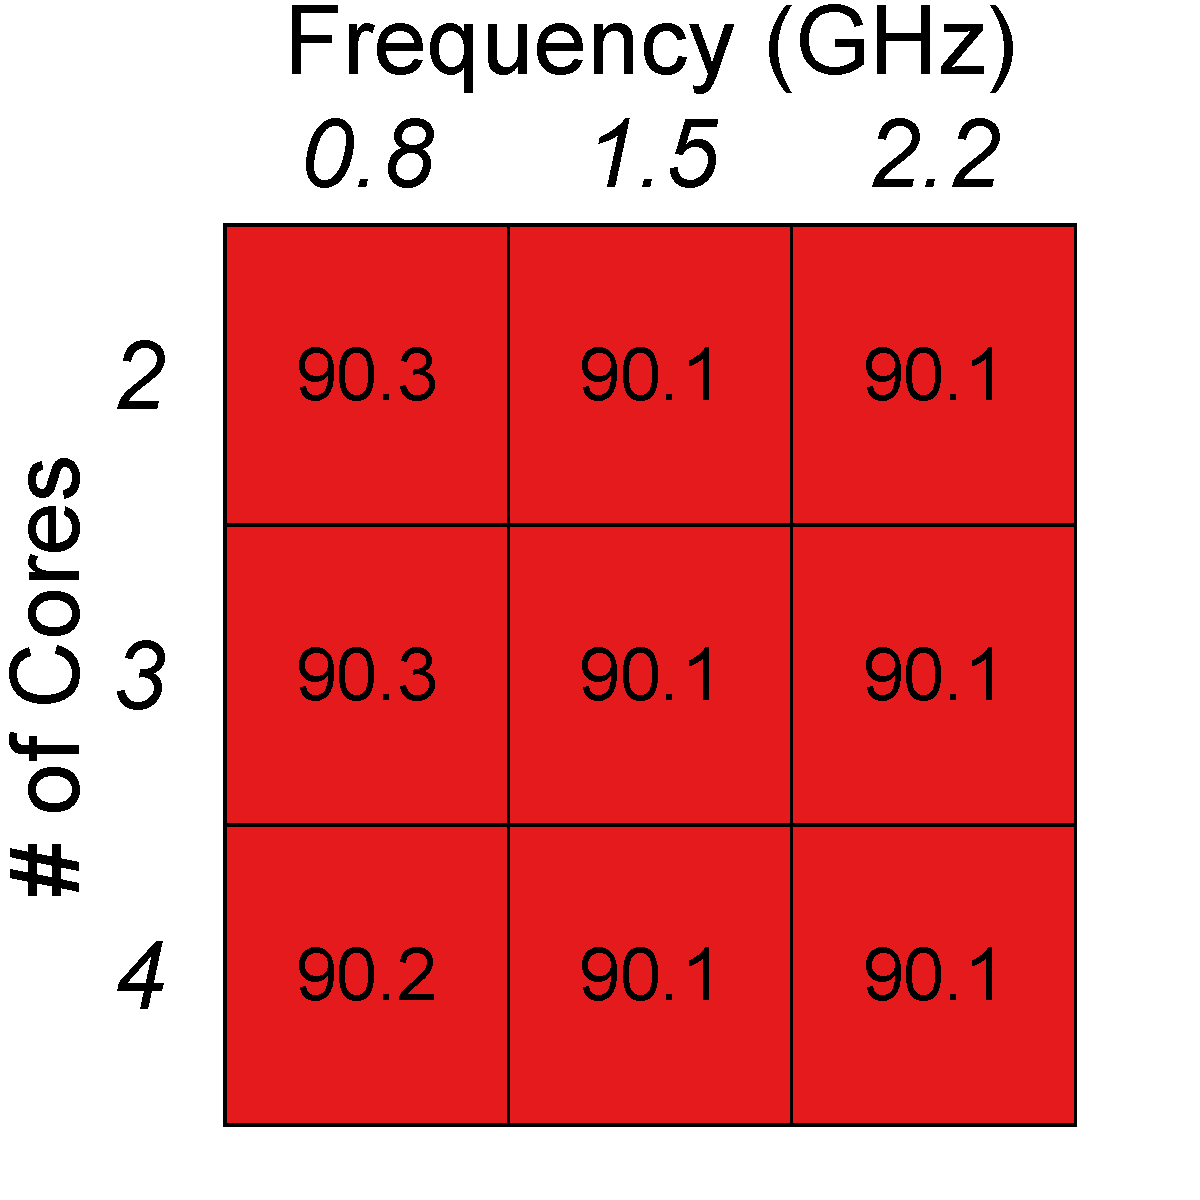
\includegraphics[width=\columnwidth]{figs/scanning_flight_time_operating_point}
    \caption{Mission Time (s)}
    \label{fig:benchmarks:OPA:scanning:time}
    \end{subfigure}
    \begin{subfigure}[t!]{.3\columnwidth}
    \centering
    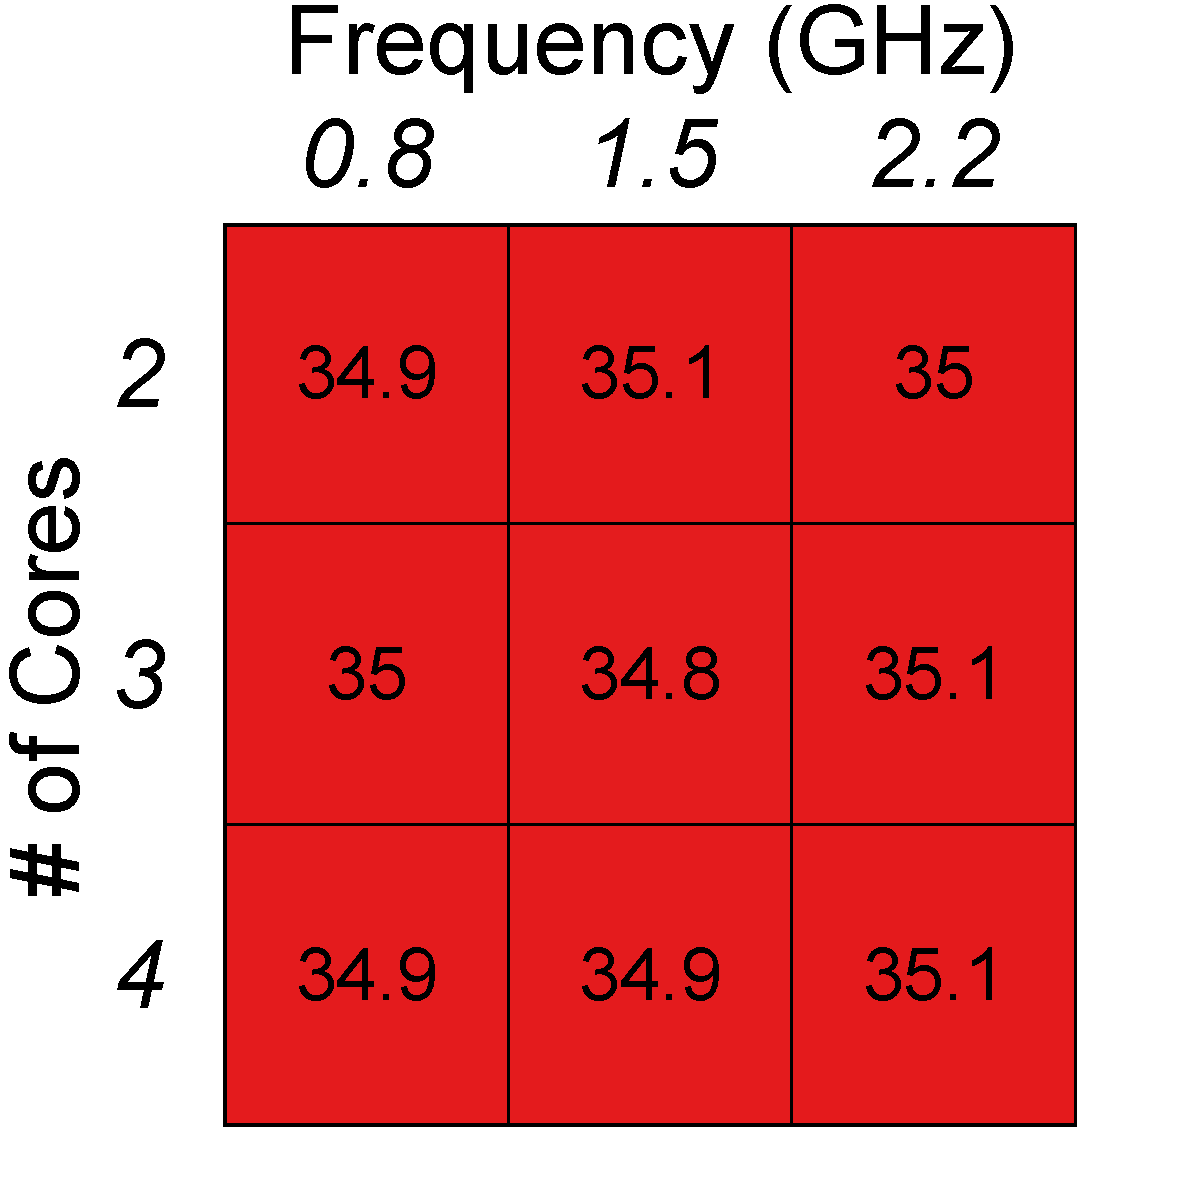
\includegraphics[width=\columnwidth] {figs/scanning_energy_operating_point}
    \caption{Energy (kJ)}
    \label{fig:benchmarks:OPA:scanning:energy}
    \end{subfigure}
    \caption{Scanning.}
    \label{fig:benchmarks:OPA:scanning}
    \end{figure}%
   \begin{figure}[t!]
    \centering
    \begin{subfigure}[t!]{.3\columnwidth}
    \centering
    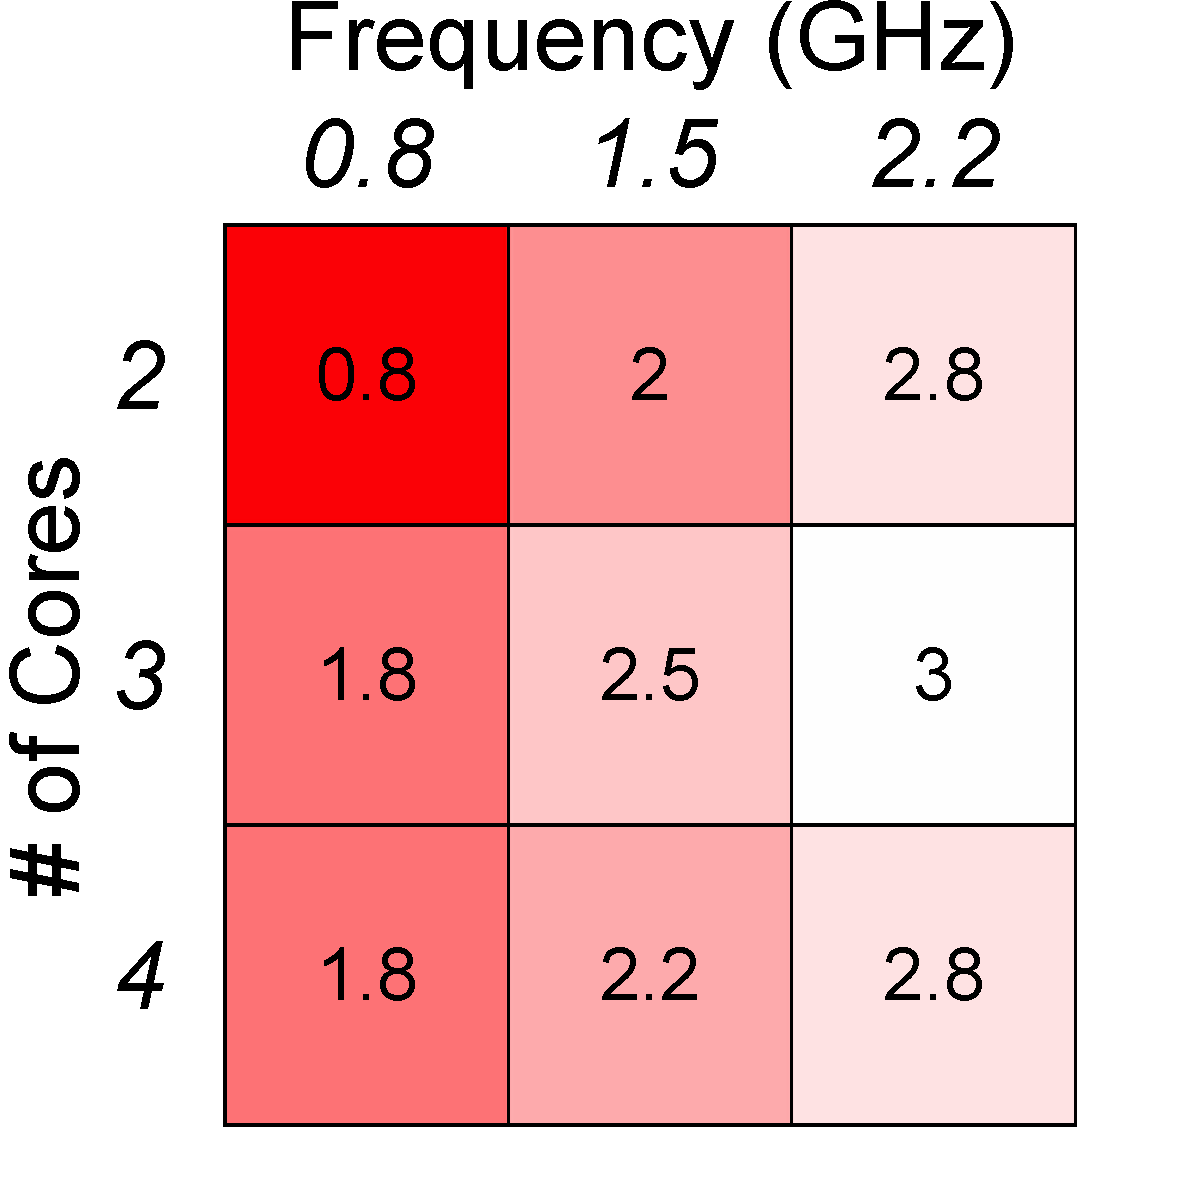
\includegraphics[width=\columnwidth]{figs/pd_velocity_operating_point}
    \caption{Velocity (m/s)}
     \label{fig:benchmarks:OPA:pd:velocity}
    \end{subfigure}
    \begin{subfigure}[t!]{.3\columnwidth}
    \centering
    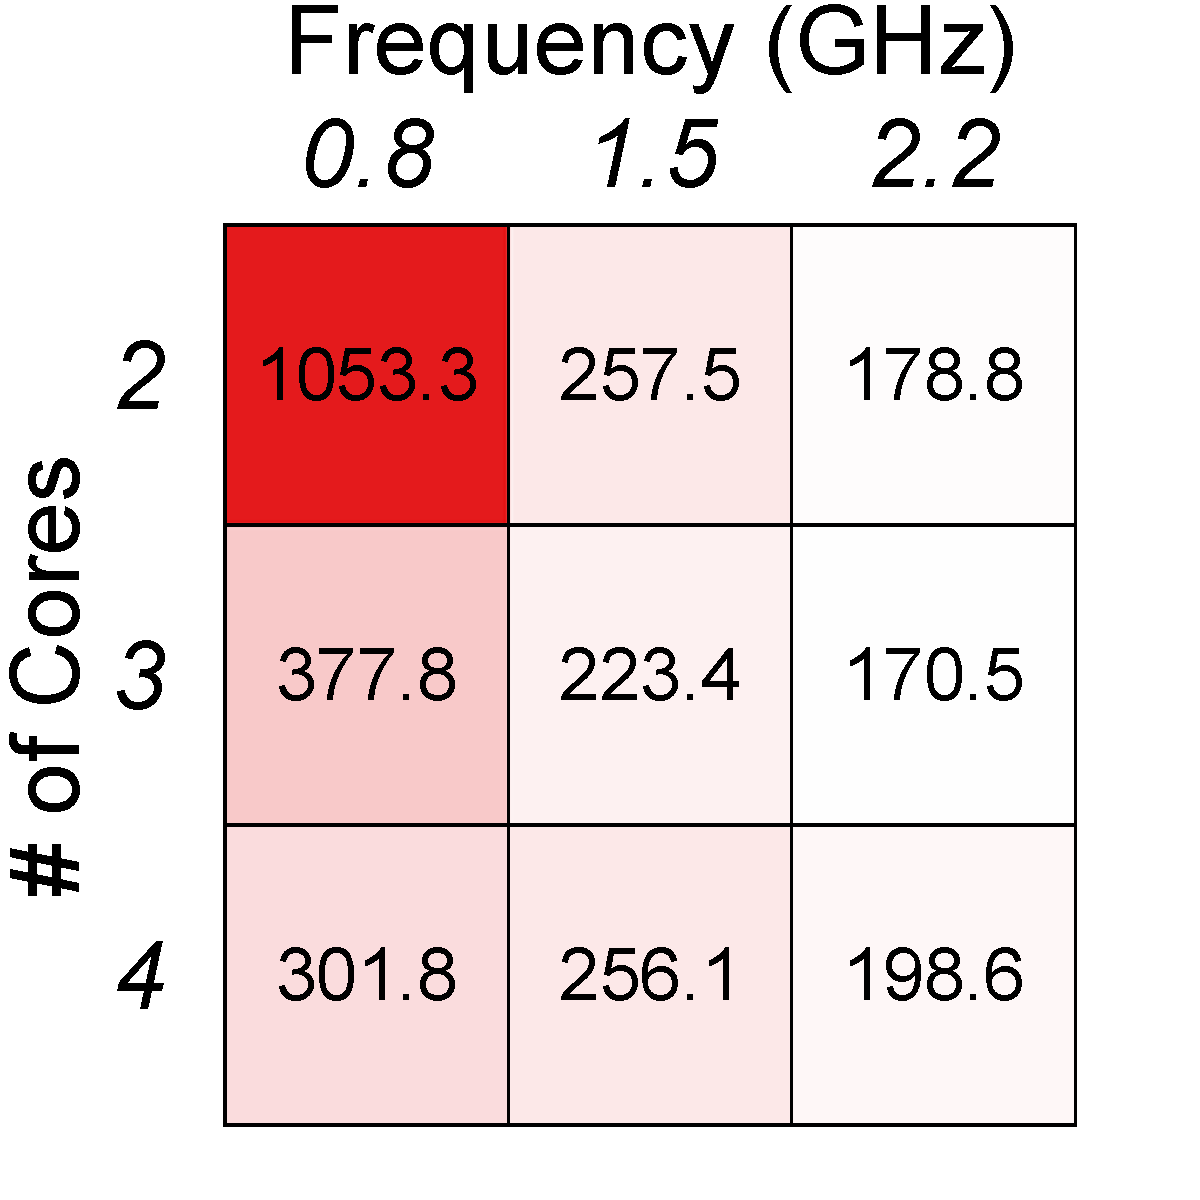
\includegraphics[width=\columnwidth]{figs/pd_flight_time_operating_point}
    \caption{Mission Time (s)}
    \label{fig:benchmarks:OPA:pd:time}
    \end{subfigure}
    \begin{subfigure}[t!]{.3\columnwidth}
    \centering
    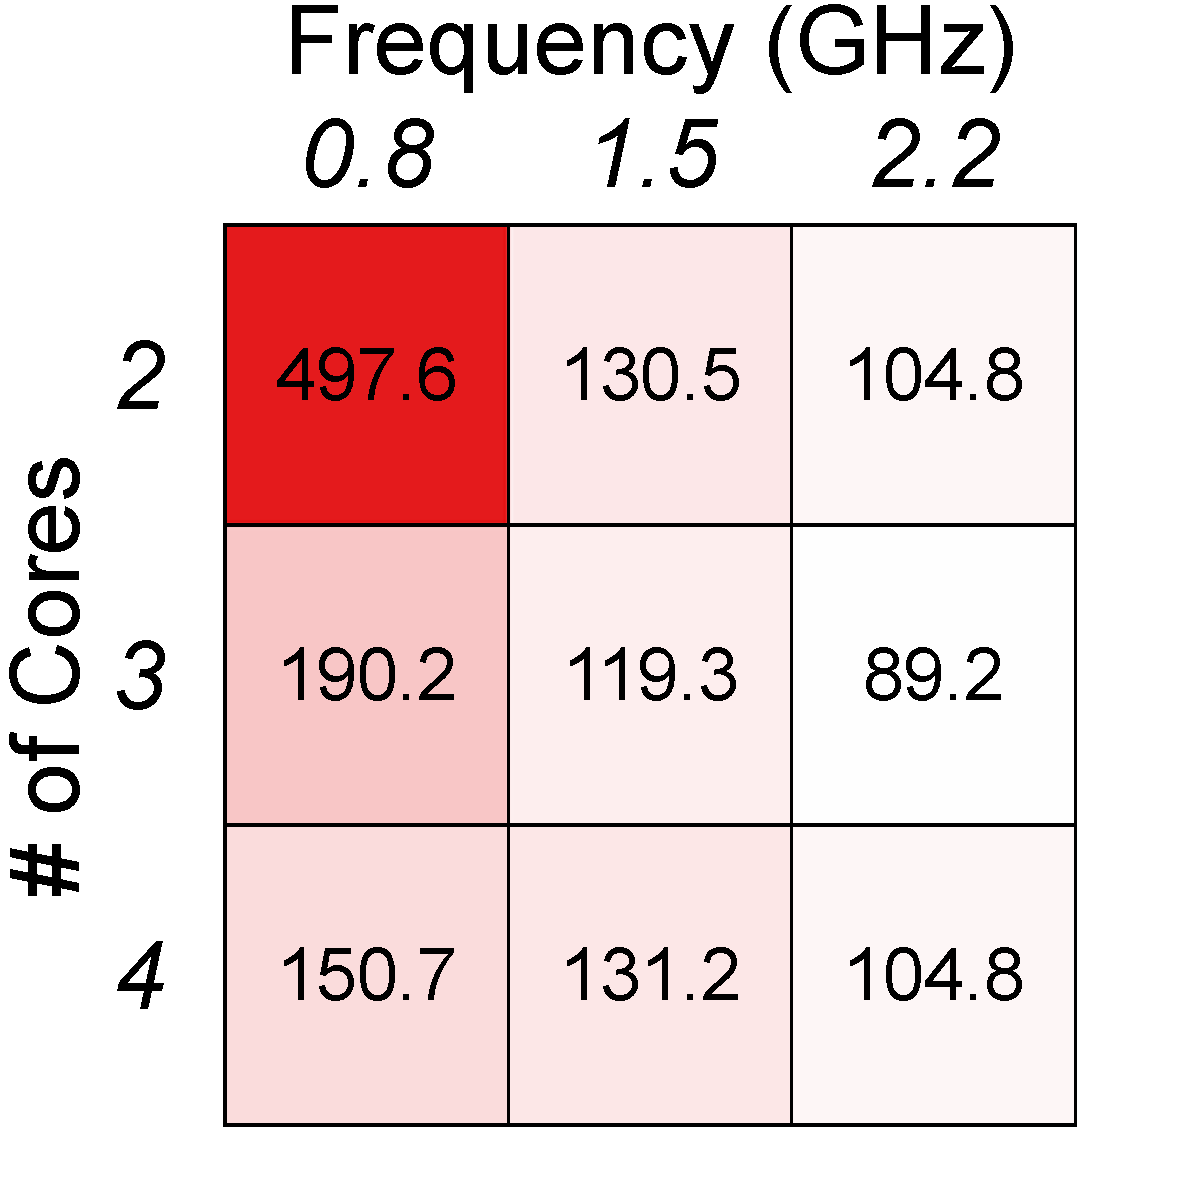
\includegraphics[width=\columnwidth] {figs/pd_energy_operating_point}
    \caption{Energy (kJ)}
     \label{fig:benchmarks:OPA:pd:energy}
    \end{subfigure}
    \caption{Package Delivery.}
    \label{fig:benchmarks:OPA:pd}
    \end{figure}%
    \begin{figure}[t!]
    \centering
    \begin{subfigure}[t!]{.3\columnwidth}
    \centering
    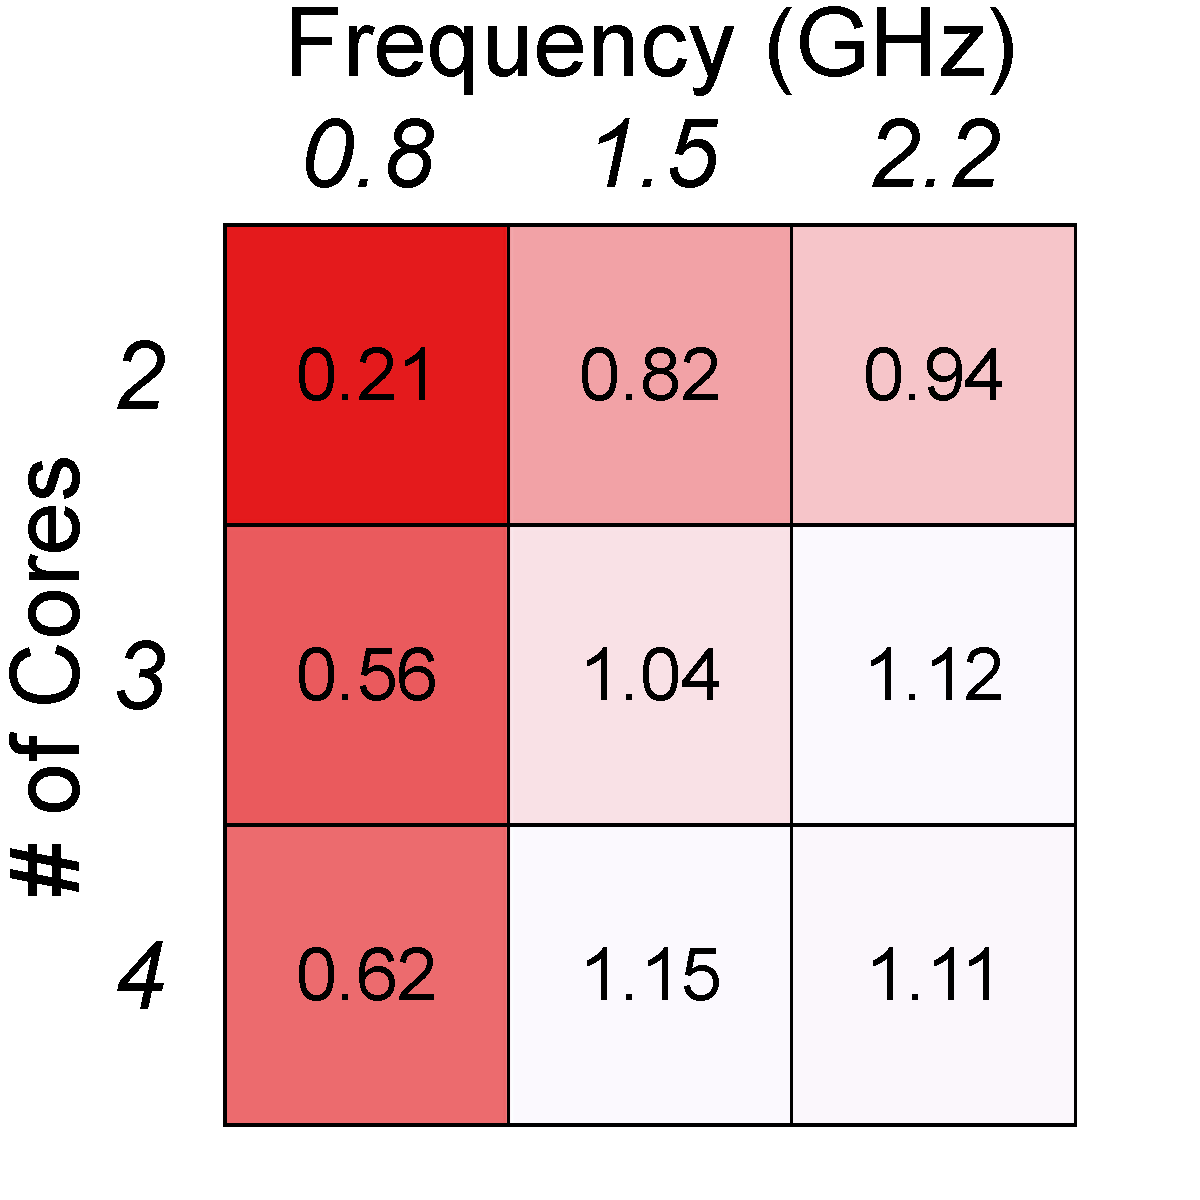
\includegraphics[width=\columnwidth]{figs/mapping_velocity_operating_point}
    \caption{Velocity (m/s)}
     \label{fig:benchmarks:OPA:mapping:velocity}
    \end{subfigure}
    \begin{subfigure}[t!]{.3\columnwidth}
    \centering
    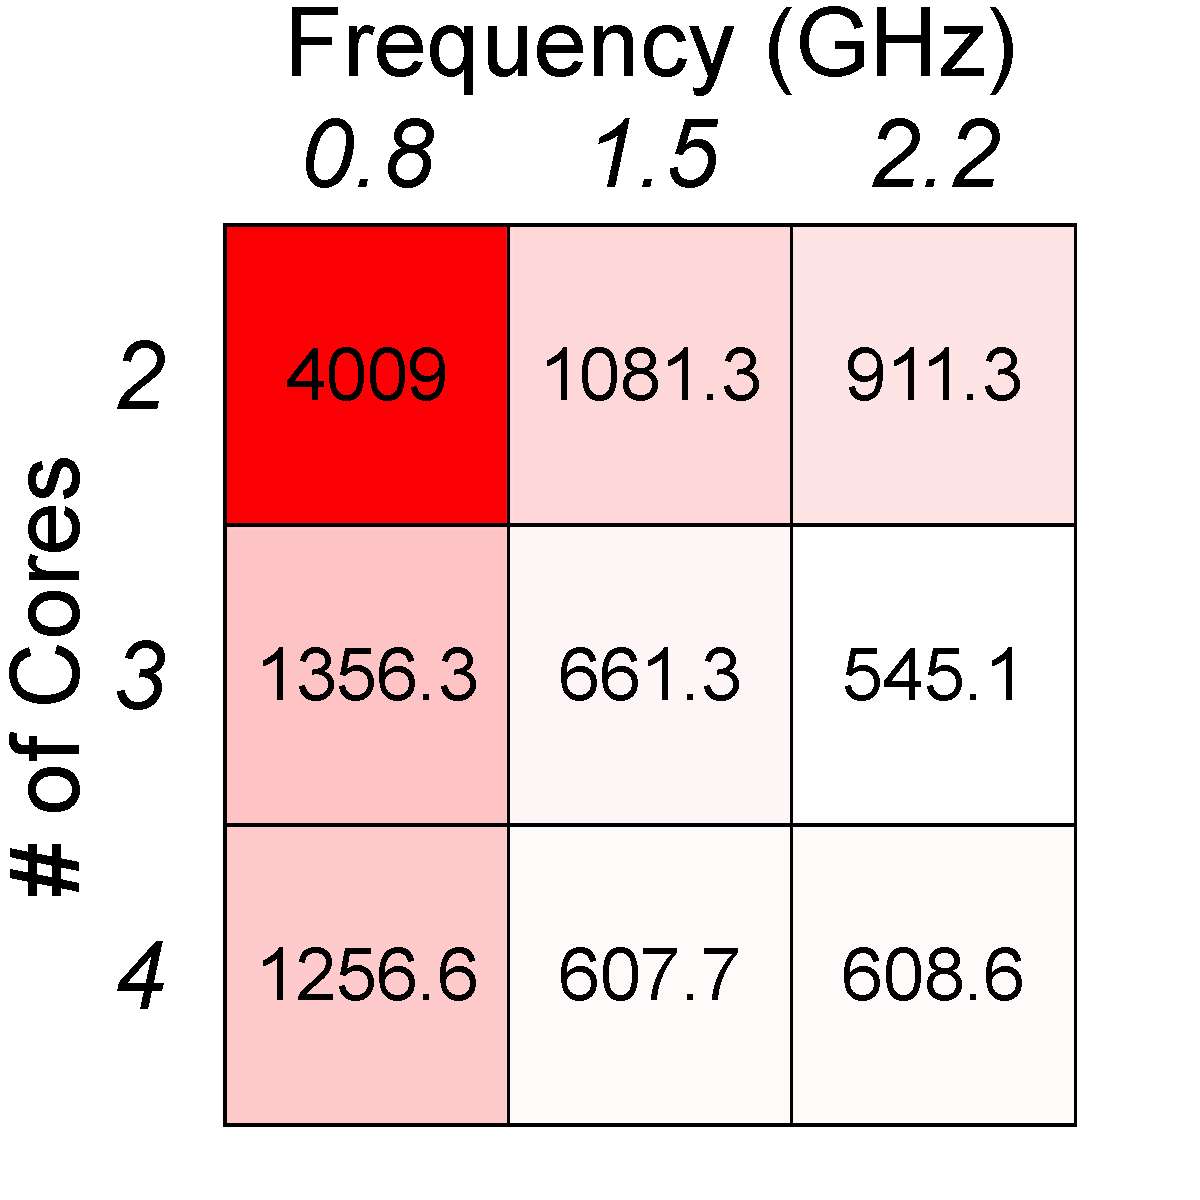
\includegraphics[width=\columnwidth]{figs/mapping_flight_time_operating_point}
    \caption{Mission Time (s)}
    \label{fig:benchmarks:OPA:mapping:time}
    \end{subfigure}
    \begin{subfigure}[t!]{.3\columnwidth}
    \centering
    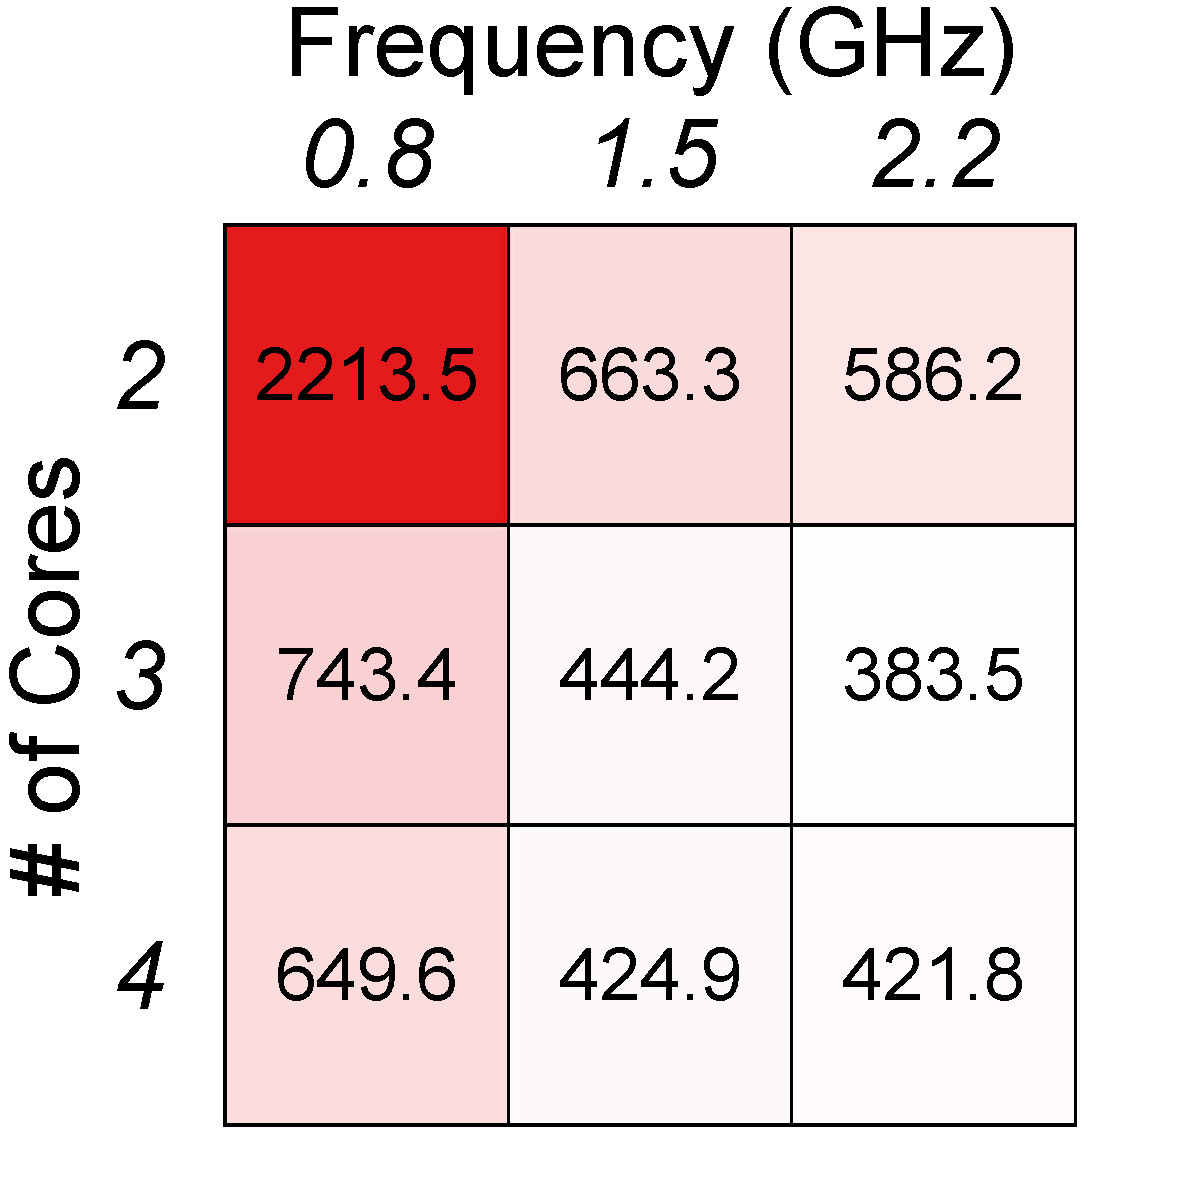
\includegraphics[width=\columnwidth] {figs/mapping_energy_operating_point}
    \caption{Energy (kJ)}
     \label{fig:benchmarks:OPA:mapping:energy}
    \end{subfigure}
    \caption{Mapping.}
    \label{fig:benchmarks:OPA:mapping}
    \end{figure}%
    \begin{figure}[t!]
    \centering
    \begin{subfigure}[t!]{.3\columnwidth}
    \centering
    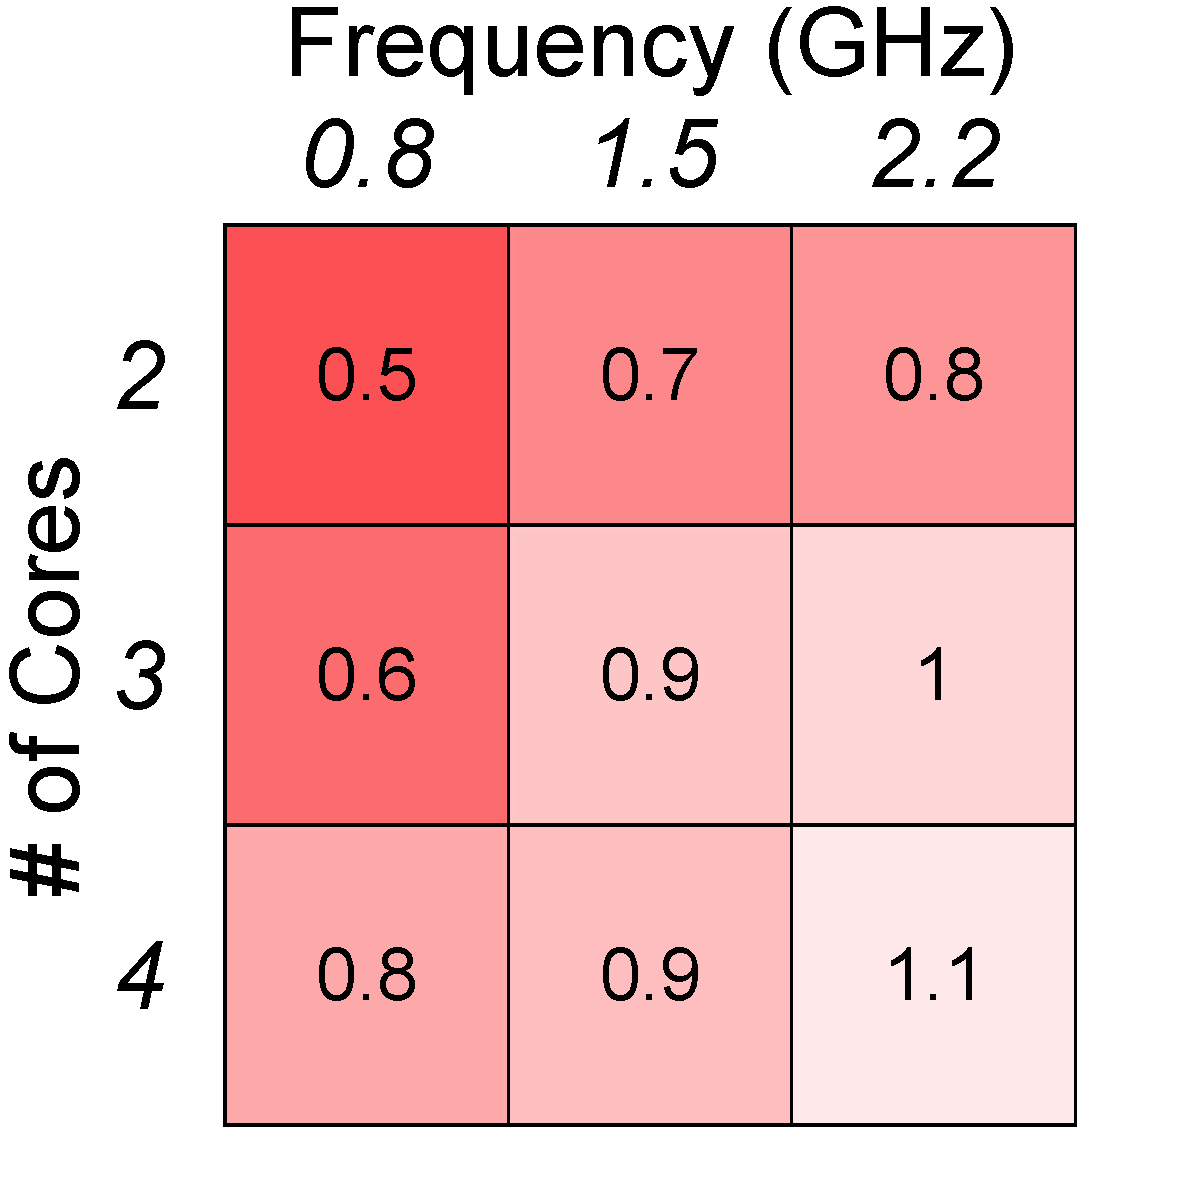
\includegraphics[width=\columnwidth]{figs/SAR_velocity_operating_point}
    \caption{Velocity (m/s)}
     \label{fig:benchmarks:OPA:sar:velocity}
    \end{subfigure}
    \begin{subfigure}[t!]{.3\columnwidth}
    \centering
    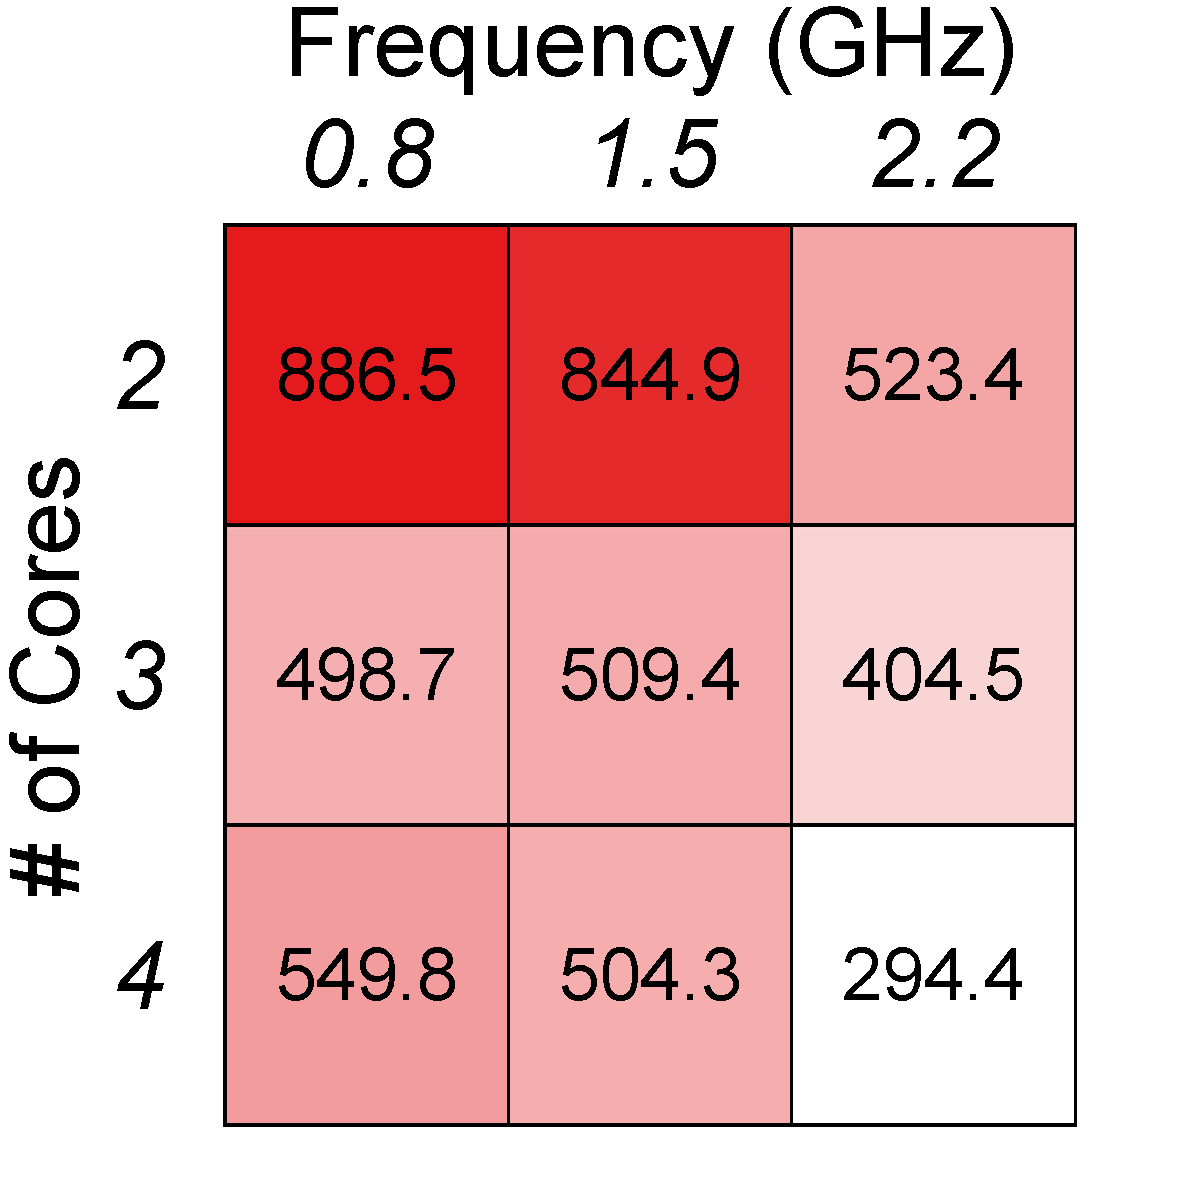
\includegraphics[width=\columnwidth]{figs/SAR_flight_time_operating_point}
    \caption{Mission Time (s)}
    \label{fig:benchmarks:OPA:sar:time}
    \end{subfigure}
    \begin{subfigure}[t!]{.3\columnwidth}
    \centering
    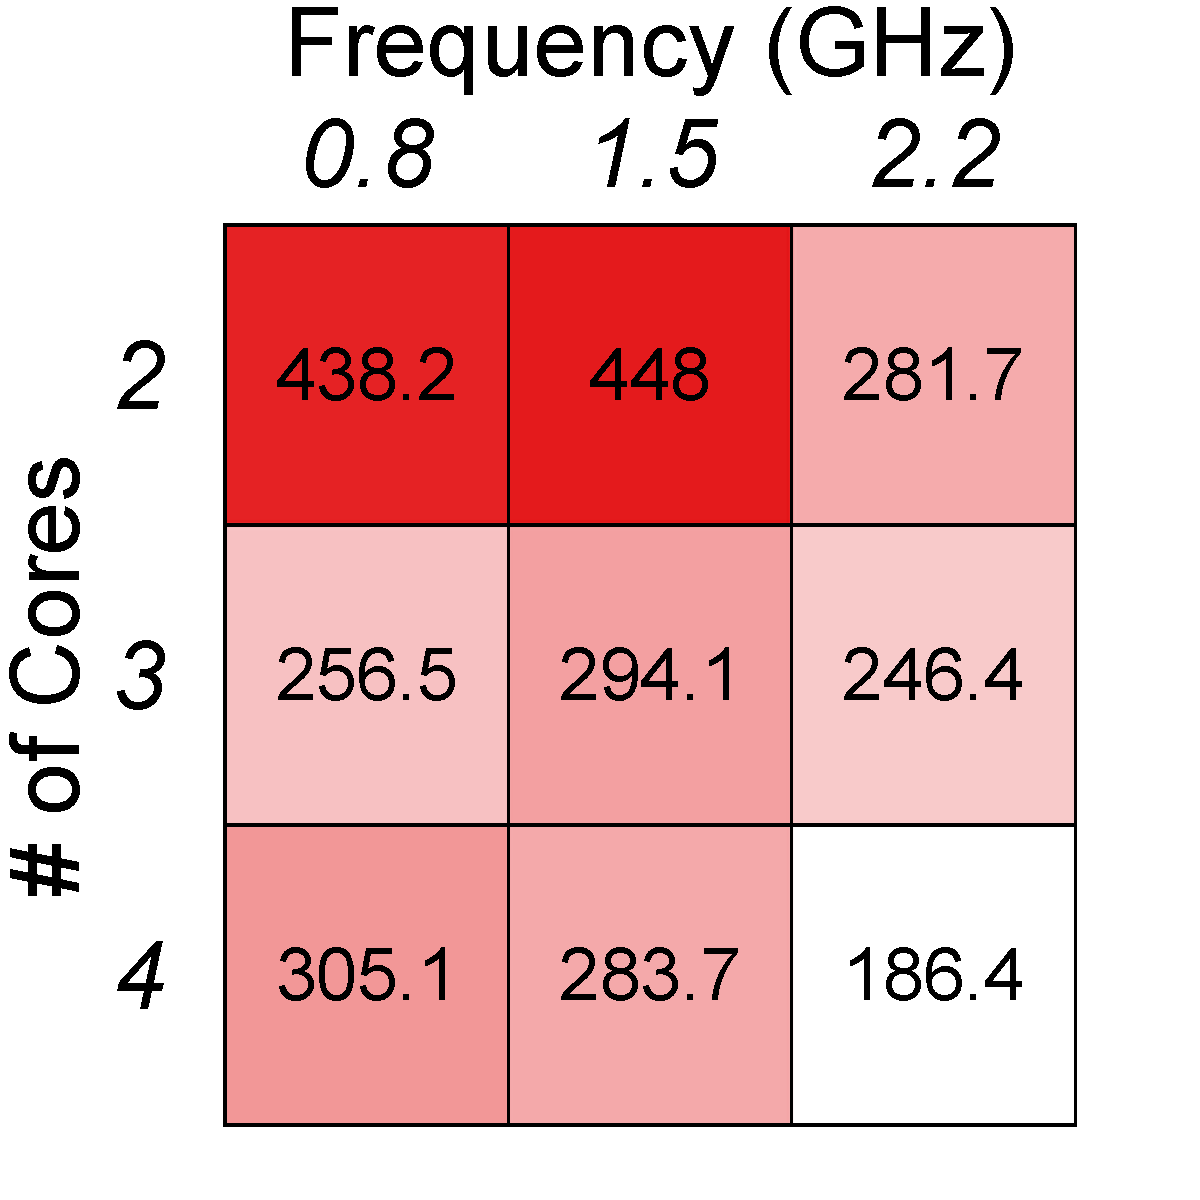
\includegraphics[width=\columnwidth] {figs/SAR_energy_operating_point}
    \caption{Energy (kJ)}
     \label{fig:benchmarks:OPA:sar:energy}
    \end{subfigure}
    \caption{Search and Rescue.}
    \label{fig:benchmarks:OPA:sar}
    \end{figure}
    \begin{figure}[t!]
    \centering
    \begin{subfigure}[t!]{.3\columnwidth}
    \centering
    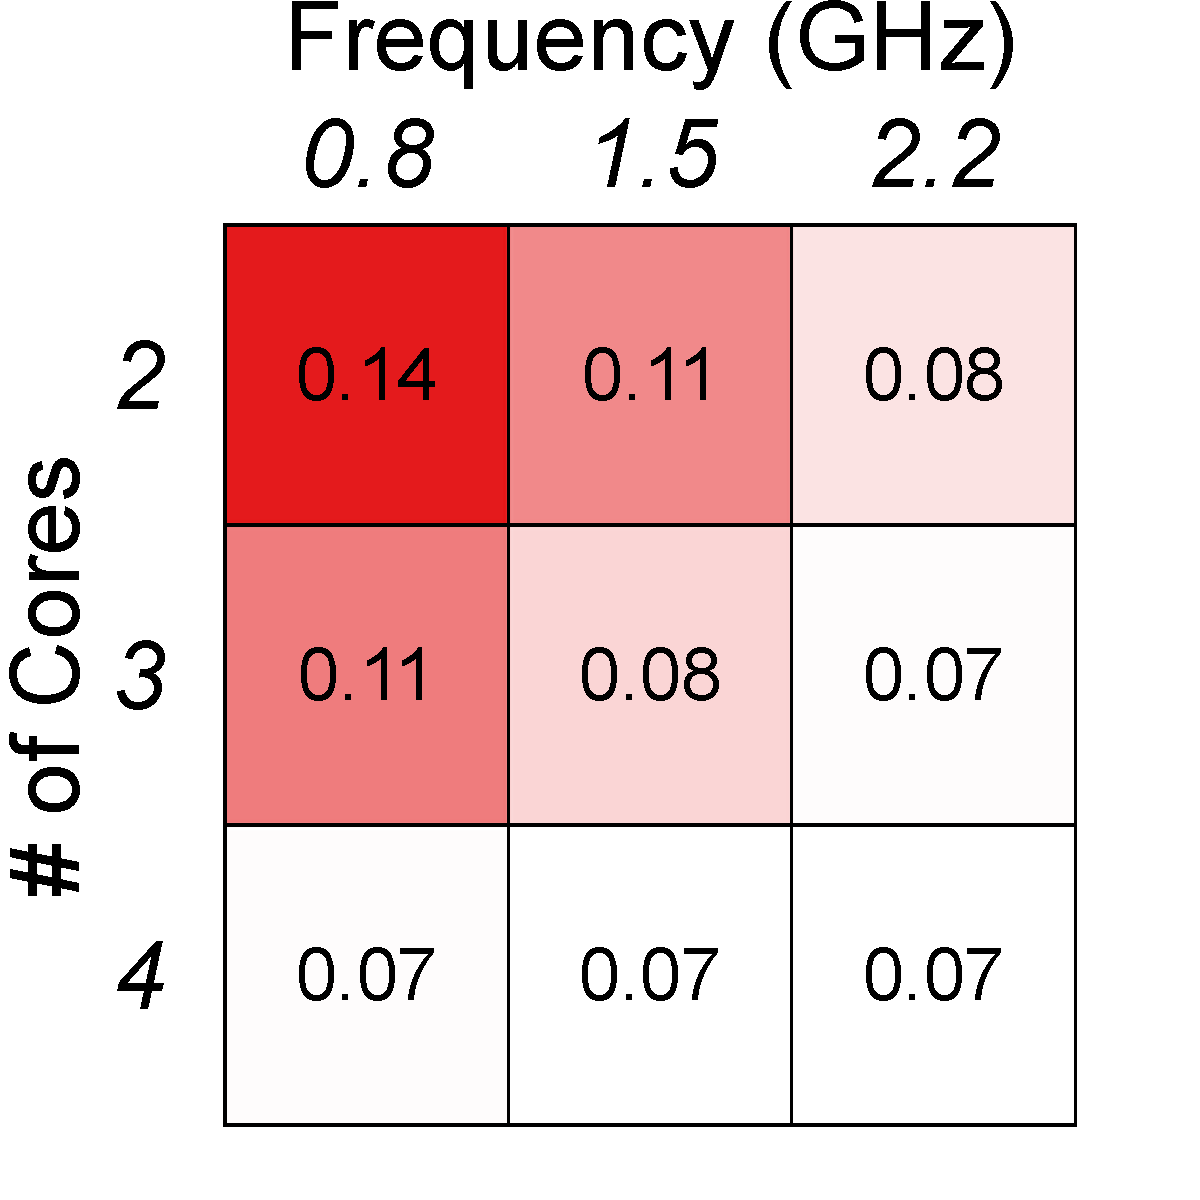
\includegraphics[width=\columnwidth]{figs/aerial_photography_error_operating_point}
    \caption{Error Rate(m/s)}
     \label{fig:benchmarks:OPA:ap:velocity}
    \end{subfigure}
    \begin{subfigure}[t!]{.3\columnwidth}
    \centering
    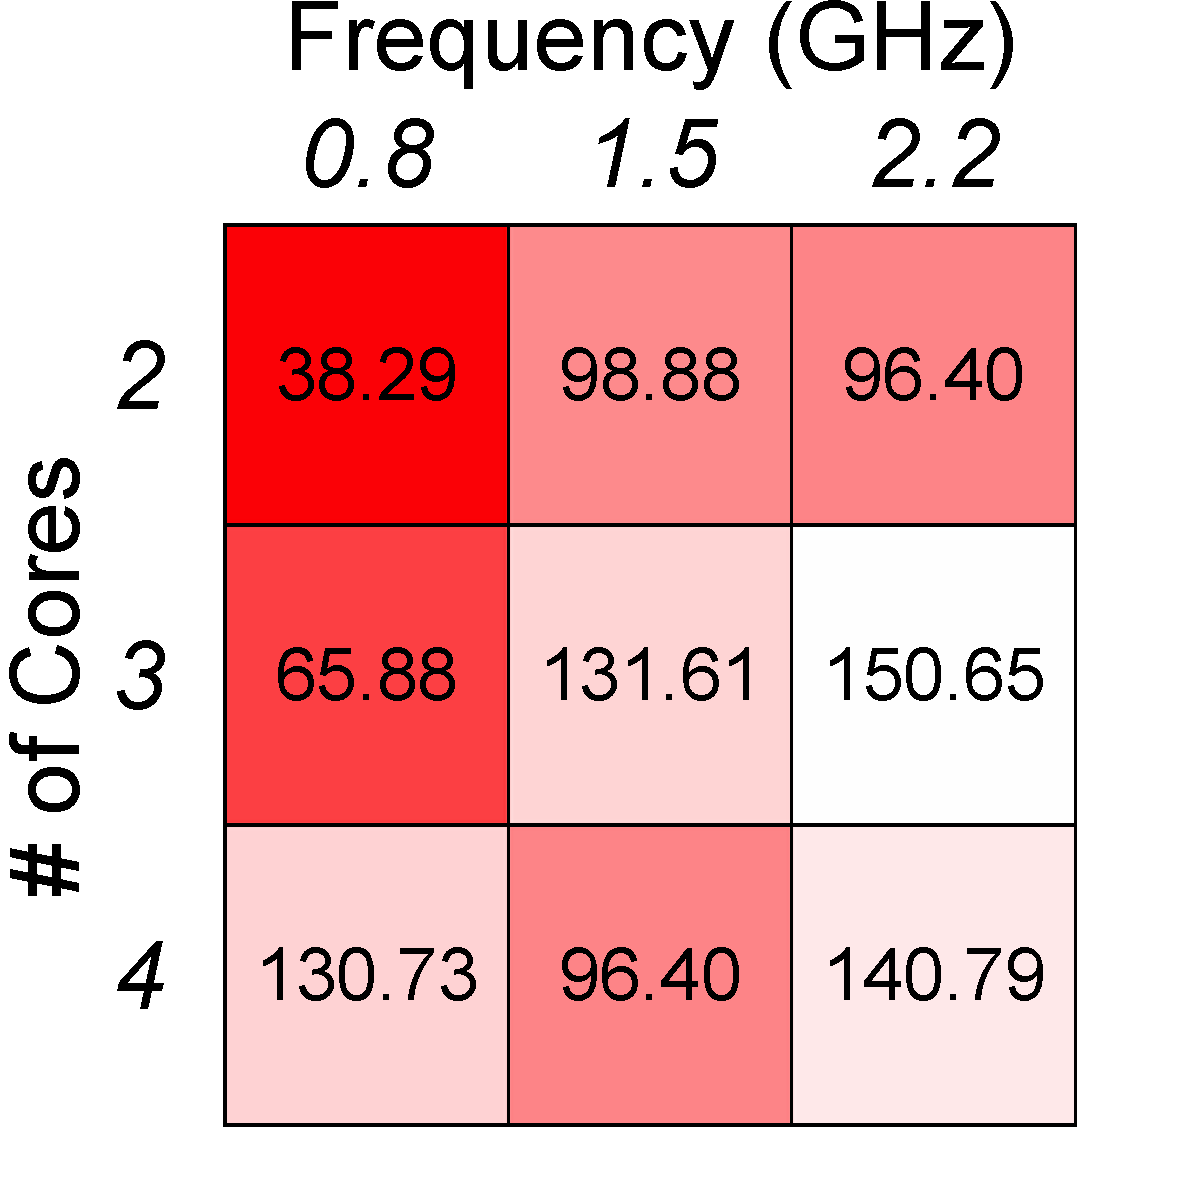
\includegraphics[width=\columnwidth]{figs/aerial_photography_flight_time_operating_point}
    \caption{Mission Time(s)}
    \label{fig:benchmarks:OPA:ap:time}
    \end{subfigure}
    \begin{subfigure}[t!]{.3\columnwidth}
    \centering
    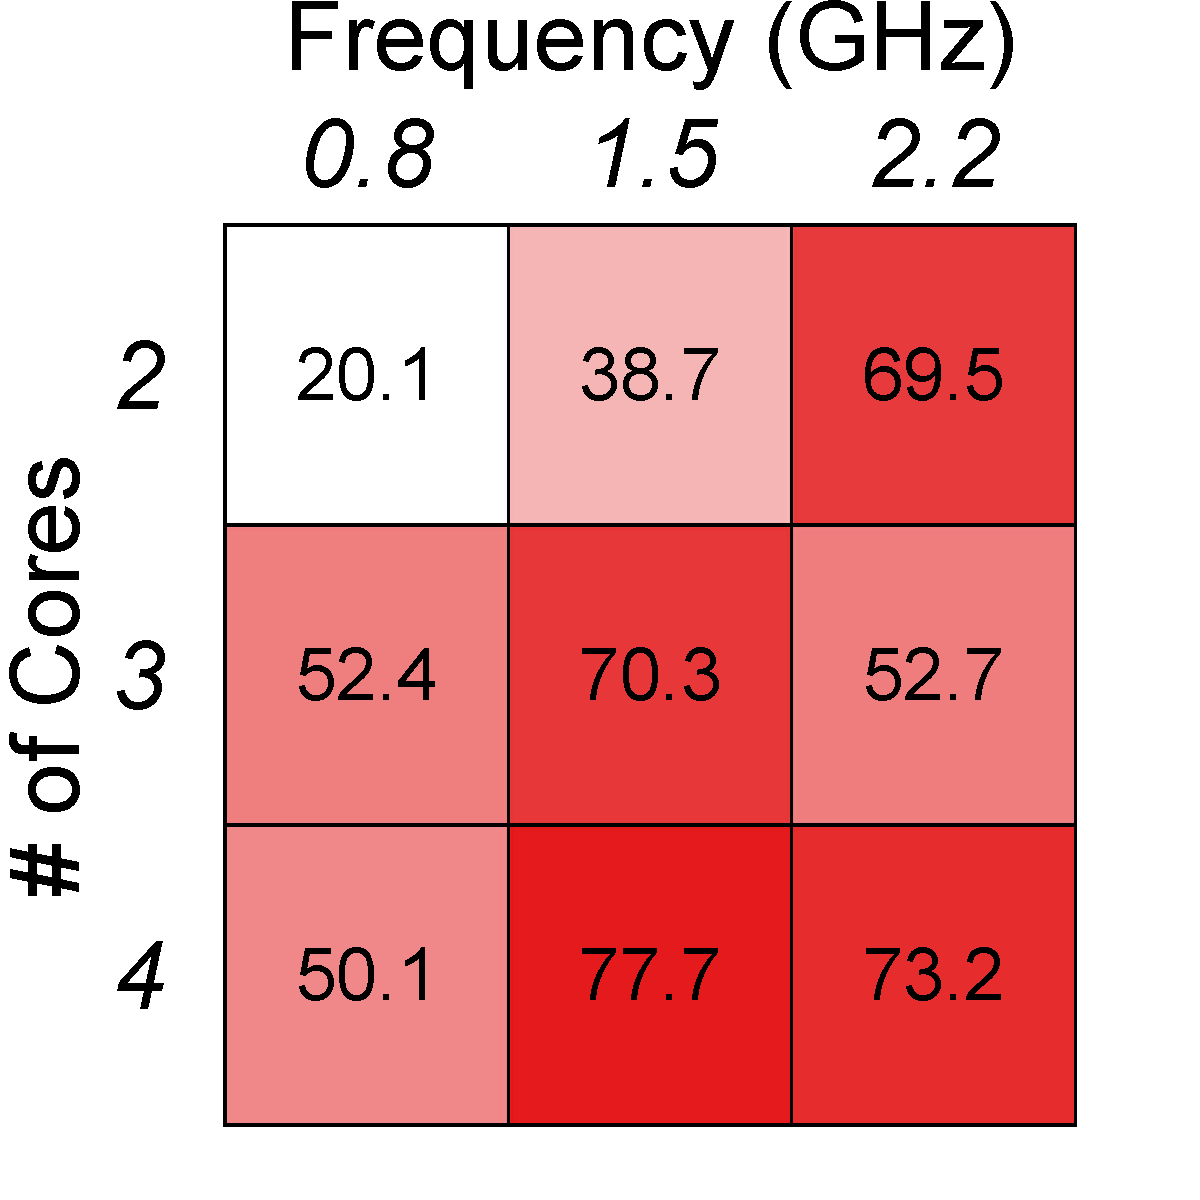
\includegraphics[width=\columnwidth] {figs/aerial_photography_energy_operating_point}
    \caption{Energy (kJ)}
     \label{fig:benchmarks:OPA:ap:energy}
    \end{subfigure}
    \caption{Aerial Photography.}
    \label{fig:benchmarks:OPA:ap}
\end{figure}
}


\paragraph{Mapping:} We observe a reduction of up to 86\% and 83\% for the mission time and energy consumption, respectively, as compute scales with the number of cores and/or frequency values (\Fig{fig:benchmarks:OPA:mapping:velocity}, \Fig{fig:benchmarks:OPA:mapping:time}, and \Fig{fig:benchmarks:OPA:mapping:energy}). The concurrency present in this application (all nodes denoted by circles with a filled arrow connection or none at all in \Fig{fig:benchmarks:data-flow:mapping} run in parallel) justifies the performance boost from core scaling. The sequential bottlenecks, i.e. motion planning and OctoMap generation explains the frequency scaling improvements. We achieve up to 6.3X improvement in motion planning (\Fig{fig:kernel-breakdown}) and that leads to hover time reduction. We achieve a 6X improvement in OctoMap generation and that leads to maximum velocity improvement. The improvements translate to a 5.3X improvement in average velocity. Since mission time is reduced, total energy consumption reduces.


\paragraph{Search and Rescue:} We see a reduction of up to 67\% and 57\% for the mission time and the energy, respectively, as compute scales (\Fig{fig:benchmarks:OPA:sar:velocity}, \Fig{fig:benchmarks:OPA:sar:time}, and \Fig{fig:benchmarks:OPA:sar:energy}). Similar to mapping, more compute allows for the reduction of hover time and an increase in maximum velocity which contribute to the overall reduction in mission time and energy. In addition, a faster object detection kernel prevents the drone from missing sampled frames during any motion. We achieve up to 1.8X, 6.8X, and 6.6X speedup for the object detection, motion planning and OctoMap generation kernels, respectively. In aggregate, these improvements translate to 2.2X improvement in the MAV's average velocity.

\begin{comment}
\begin{figure}[!t]
\centering
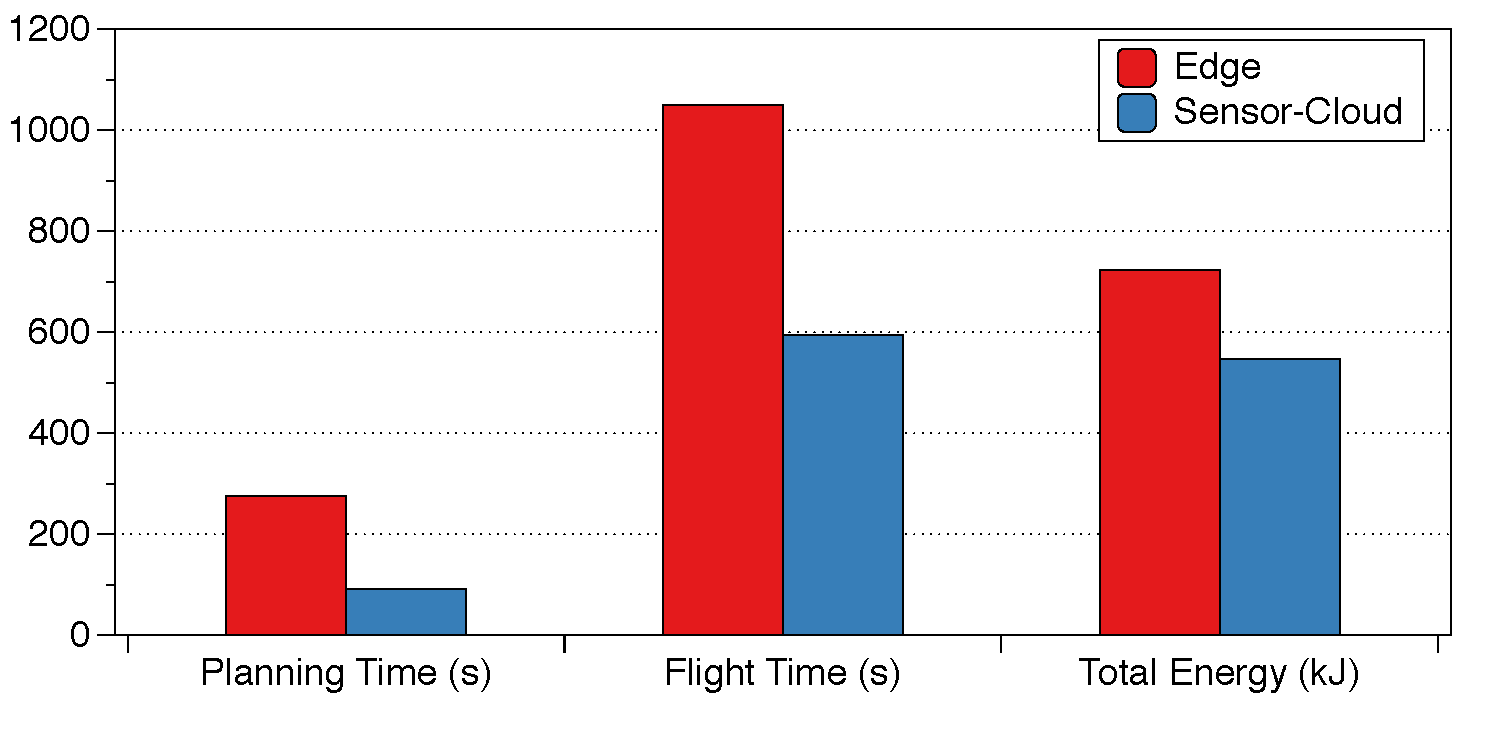
\includegraphics[trim=0 0 0 -25, clip, width=0.9\linewidth]{figs/tx2-desktop}
\vspace{-12pt}
\caption{Comparing a full-on-edge drone versus a full-on-cloud drone. Our system allows part or portion of the MAVBench workloads to be offloaded to the cloud (or another local co-processing agent).}
\label{fig:cloud_edge}
\end{figure}
\end{comment}

\paragraph{Aerial Photography:} We observe an improvement of up to 53\% and 267\% for \emph{error} and mission time, respectively (\Fig{fig:benchmarks:OPA:ap:velocity}, \Fig{fig:benchmarks:OPA:ap:time}, and  \Fig{fig:benchmarks:OPA:ap:energy}). In aerial photography, as compared to other applications, higher mission time is more desirable than a lower mission time. The drone only flies while it can track the person, hence a longer mission time means that the target has been tracked for a longer duration. In addition to maximizing the mission time, error minimization is also desirable for this application. We define error as the distance between the person's bounding box (provided by the detection kernel) center to the image frame center.  Clock and frequency improvements translate to 2.49X and 10X speedup for the detection and tracking kernels and that allows for longer tracking with a lower error. No significant trend is observed in the energy data because energy depends on both the mission time and the velocity, and as opposed to the other applications, there is no need for the drone to minimize its velocity. Instead, it needs to successfully track the person.


\begin{figure*}[!t]
\centering
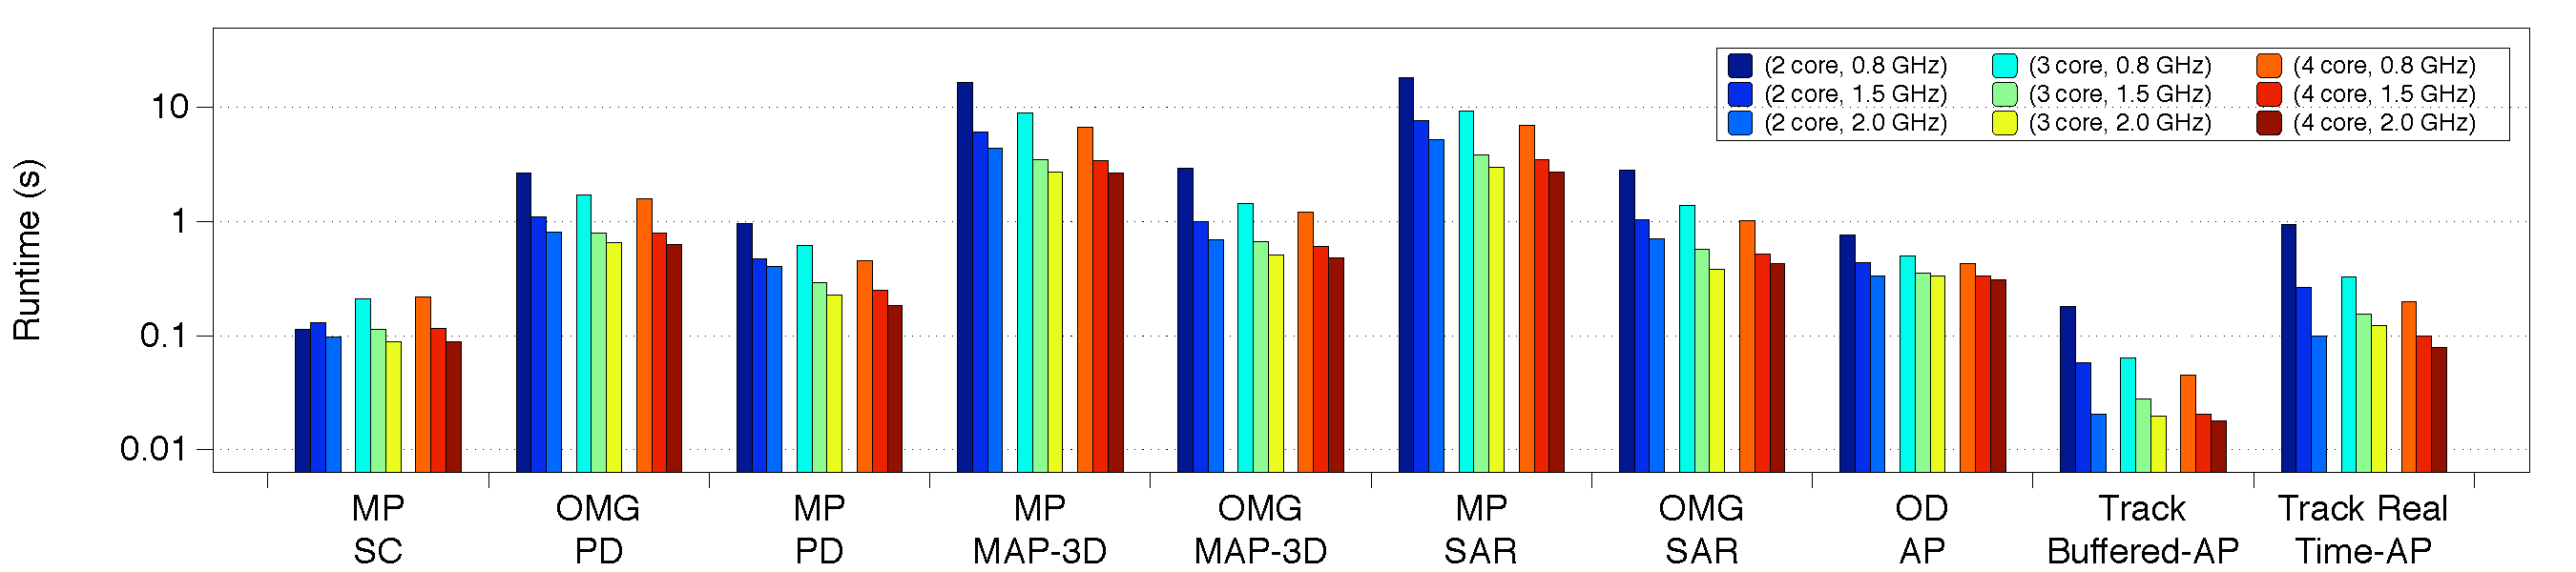
\includegraphics[width=\columnwidth]{figs/kernel-breakdown_2}
\vspace{-18pt}
\caption{Kernel breakdown for MAVBench. The abbreviations are as follows: \emph{OD-}Object detection, \emph{MP-}Motion Planning, \emph{OMG-}OctoMap Generation for kernels and \emph{SC-}Scanning, \emph{PD-}Package Delivery,  \emph{MAP-}3D Mapping, \emph{SAR-}Search and Rescue, and \emph{AP-}Aerial Photography for applications. The $x$-axis lists the kernel-application names and $y$-Axis represents the runtime in seconds. Each bar graph represents one of the configurations used in the hardware. The cores are varied from 2 to 4 and the frequency goes from from 0.8 GHz , 1.5 GHz or 2.2 GHz.}
\label{fig:kernel-breakdown}
\end{figure*}

%\begin{minipage}[!]{0.99\columnwidth}
   
%\end{minipage}


%In the perception stage of this application, a person is detected, and the bounding box associated with the person is tracked. The tracking stage consists of two nodes itself. The first node (buffer then track) buffers the images while detection is running and then track the buffered once the person is detected. The second node (track continuously) tracks the previous bounding box while the new one is calculated. Buffer then track node is necessary, since otherwise, image difference between the image detection sampled and tracking is large enough that increases the false positive tracking. PID node calculates the difference between the targets place and where it should be in the frame and sends small trajectories to the drone. Similar to other applications, these trajectories are followed in the follow trajectory node.

%Compute's effect on this application is on its accuracy and the duration in which drone can follow the target. In other words, faster compute can affect how closely and for how long the target is tracked. 
%\subsection{Understanding the Compute to Endurance Relationship}
%in this section, we demonstrate the relationship between compute on the drone and the drone's mission time (i.e., endurance). We start by showing that looking naively indicates that compute consumes an insignificant amount of power, and that much of the power is spent on keeping the drone afloat using its rotors. Therefore, this leads to a shortsighted conclusion that compute does not play a dominant role in autonomous flight for dron

%\subsection{Micro architectural characterization}
%To understand the reason behind the aforementioned bottlenecks, we provide micro-architectural characterization of them. This will help the designers to design for the future MAV systems while alleviating such bottlenecks. Our analysis show that the bottle necks mainly exists in the perception and the planning stage. Hence, we turn our focus solely to these two stages.  
%
%characterize OctoMap, slam and nbvPlanner. 

\begin{comment}
%\subsubsection{Algorithmic Choices}
%Algorithms at some point will be general enough to cover all the environments, hence we shouldn't 
%be highlighting our algorithmic sensitivity to environment (which in this argument is considered in a flaw)
 
\subsection{explanation of each apps inter kernel interactions}
\textbf{Scanning:} This application involves only a single ROS node. All the code runs on a CPU, with no parallelization. The main computational kernel is the simple path-planning since no collision-checking is involved. This is because the \textit{Scanning} benchmark is meant for outdoors environments, high aboveground where obstacles are not to be found. Because the benchmark is meant for outdoors environments, localization is accomplished through the use of GPS sensors, which incur negligible computational overhead.

\textbf{Aerial Photography}
This application involves three ROS nodes running concurrently. One node is responsible for running object detection algorithms to locate the human target. However, object detection is normally a very computationally-intensive task that can take up to several seconds to complete. Therefore, another node runs much faster tracking algorithms such as KCF which estimate the position of the target in the interval between completions of the object detection algorithm. Another node controls the motion of the MAV based on the position of the target. All nodes run on the CPU except for the object detection node which runs on a GPU.

\textbf{Package delivery:}
This application involves 4 ROS nodes, which all run on CPU cores. One node plans collision-free trajectories using the path-planning algorithms described in the previous section. Another node waits for paths to be planned and then controls the motion of the MAV to follow them. However, as the MAV follows these trajectories, it may uncover new obstacles in its environment that had been out of range of its sensors when the path was initially planned. Therefore, an additional node must constantly run to check whether any newly uncovered obstacle causes a collision upon the planned trajectory, so that the path can be re-planned if necessary. Finally one final node must provide localization capabilities, either through GPS or SLAM, to enable the MAV to follow its planned trajectory accurately.

\textbf{Mapping}
This application involves 3 ROS nodes which all run on CPU cores. One node samples its environment and finds points on the boundary of previously explored space where the MAV can be expected to maximize the amount of unknown space that it uncovers. Once these points are found, the node then plans a path towards them along an RRT tree. A second node controls the motion of the MAV, following the trajectories generated by the first node. Finally, a third node must provide localization, such as through SLAM. This localization must be accurate, because the MAV updates its internal map based upon the position it believes it is in. If the MAV relies upon an inaccurate SLAM algorithm, the map it generates may not be completely accurate.


\textbf{Exploration:}
Computationally, this application includes the same nodes as the \textit{Exploration} benchmark, as well as another node that constantly runs object detection algorithms to search for human victims as it explores unknown environments. The object detection node here runs on a GPU. The object detection algorithm must run fast, in order to allow the MAV to sweep a large area quickly, but they must also be highly accurate, to prevent the MAV from missing a victim due to a false negative.


\label{sec:characterization}
 possibly the bottlenecks, and a table with kernel times and their distribution.
 
 possibly the requirements compute wise and which platforms are suitable for them (refer back to the HIL and how we can conduct these conclusive studies)

\subsection{Environment and it's effects}
indoor/outdoor,
obstacle density, dynamic obstacle speed
\subsection{}

\end{comment}

 
